%==============================================================================    
\chapter{Front-end electronics}
\label{sec:FE_electronics}
%==============================================================================    

One of the key components of the detector systems is the readout
electronics. Each experiment, depending on the requirements, has its
own specific electronics. But the basic principles of the electronics
and optimisations of the signal-to-noise remain similar between
different applications.

\section{Basic principles}

The main purpose of the detecting system is to acquire the signal
generated in the sensor which is in the form of a short current
pulse. The electronics are responsible for shaping the time response
of the system in order to optimise the minimum detectable signal,
energy deposition in detector measurement, event rate, time-of-arrival
and insensitivity to the pulse shape. Finally, the signal is digitised
and stored. Robustness to radiation and power consumption are other
important considerations to be addressed amongst others.

\cref{fig:detectorFunctions} schematically overviews the basic
detector functions. The incident radiation deposits energy in the
sensor and it is converted to an electrical signal. The sensor pulse
being very short (few nanoseconds), a high rate of particles can be
handled in a semiconductor detector. Since the magnitude of the signal
charge can be small and is subject to statistical fluctuations
(\cref{sec:chargeInSi}), a preamplifier is needed to amplify the
signal. The preamplifier should be designed in such a way to minimise
the electronic noise. The sensor capacitance and the input capacitance
of the amplifier are the critical parameters to increase the
signal-to-noise ratio (SNR): the lower the capacitance, the higher the
SNR.

After the preamplifier, the pulse shaper is responsible for the
improvement of the SNR. It modifies the frequency response of the
signal to improve the signal and attenuate the noise. Since this
operation reduces the bandwidth of the signal, the duration of the
pulse will increase. A detector must cope with a high rate of pulses,
the width of the pulse must be optimised in a way to reduce the
pile-up.

The analog-to-digital converter (ADC) converts a continuously varying
amplitude to discrete steps. When the pulse height passes a threshold
in a comparator, counters are incremented to measure the energy and
the timing of the signal for example.

\begin{figure}[htbp]
  \centering
  \begin{tikzpicture}
      \begin{scope}[x={(image.south east)},y={(image.north west)}]
        % \draw[help lines,xstep=.1,ystep=.1] (0, 0) grid (1,1);
        % \foreach \x in {0,1,...,9} { \node [anchor=north] at (\x/10,0) {0.\x}; }
        % \foreach \y in {0,1,...,9} { \node [anchor=east] at (0,\y/10)
        %   {0.\y}; }

        %\path (-0.1, 0.5) -- ++(0.08, 0.5) node[rv] {Incident radiation};
        \draw (0.1, 0.4) rectangle (0.3, 0.6) node[pos=.5] {Sensor};
        \draw (0.4, 0.6) -- (0.4, 0.4) -- (0.6, 0.5) -- cycle;
        \node[above] at (0.5, 0.65) {Preamplifier};
        \draw (0.7, 0.6) -- (0.7, 0.4) -- (0.9, 0.5) -- cycle;
        \node[above] at (0.8, 0.65) {Pulse shaping};
        \draw (1, 0.35) rectangle (1.3, 0.65) node[pos=.5] {ADC converter};
        % \node[above] at (1.15, 0.7) {Analog to digital convertor};

        \draw[arrows=->](-0.1, 0.5)--(0.08, 0.5) node [pos=0.1, above]
        {Incident radiation};

        \draw[arrows=->](0.3, 0.5)--(0.4, 0.5);
        \draw[arrows=->](0.6, 0.5)--(0.7, 0.5);
        \draw[arrows=->](0.9, 0.5)--(1, 0.5);
        \draw[arrows=->](1.3, 0.5)--(1.5, 0.5) node [pos=0.8, above]
        {Digital data bus};
        

      \end{scope}
  \end{tikzpicture}
  \caption{Schematic overview of basic detector functions.}  
  \label{fig:detectorFunctions}
\end{figure}

\cref{fig:TOT_TOA_concept} schematically shows the energy and the
timing measurement of the signal. The Time-over-threshold (TOT) allows
for the measurement of the energy deposited in a pixel. The pulse is
amplified and the pulse shaper integrates the signal to form a step
pulse with a long linear decay. The decay is approximately linear and
proportional to the energy deposited. While the pulse is above the
programmable threshold, the counter is incremented.

The Time-of-Arrival (TOA) measures the arrival time of a hit and
therefore is used as a time stamping of the hits. When the amplifier
output exceeds the pixel threshold, the discriminator output rises and
the fast TOA (FTOA) counter counts until the rising edge of the
general clock ($40\,\megahertz$).

\begin{figure}[htbp]
  \centering
  \begin{tikzpicture}
    \begin{scope}[x={(image.south east)},y={(image.north west)}]
      % \draw[help lines,xstep=.1,ystep=.1] (0, 0) grid (1,1);
      % \foreach \x in {0,1,...,9} { \node [anchor=north] at (\x/10,0) {0.\x}; }
      % \foreach \y in {0,1,...,9} { \node [anchor=east] at (0,\y/10)
      % {0.\y}; }
      
      % pulse
      \draw[-, thick] (0.1, 0.8) -- (0.2, 0.8);
      \draw[-, thick] (0.2, 0.8) -- (0.21, 0.98);
      \draw[-, thick] (0.21, 0.98) -- (0.22, 0.8);
      \draw[-, thick] (0.22, 0.8) -- (1, 0.8);

      % shaper
      \draw[-, thick] (0.1, 0.5) -- (0.2, 0.5);
      \draw[-, thick] (0.2, 0.5) -- (0.22, 0.7);
      \draw[-, thick] (0.22, 0.7) -- (0.8, 0.5);
      \draw[-, thick, dashed, green] (0.1, 0.55) -- (0.8, 0.55);
      \draw[-, thick] (0.8, 0.5) -- (1, 0.5);

      % comparator
      \draw[-, thick] (0.1, 0.3) -- (0.21, 0.3);
      \draw[-, thick] (0.21, 0.3) -- (0.21, 0.4);
      \draw[-, thick] (0.21, 0.4) -- (0.65, 0.4);
      \draw[-, thick] (0.65, 0.4) -- (0.65, 0.3);
      \draw[-, thick] (0.65, 0.3) -- (1, 0.3);

      \timing [] at (0.1,0.2) {LLLHHLLHHLLHHLLHHLLHHLLLL};
      \draw[arrows=<->, thick](0.21, 0.15)--(0.65, 0.15) node [pos=0.5, below]
      {\textbf{TOT (3 counts)}};

      \timing [] at (0.1,0.0) {llllllhlhlhlhllllllllllllllllllllllllllllllllllllll};

      \draw[-, thick, dashed, blue] (0.21, 0.55) -- (0.21, 0.0);
      \draw[-, thick, dashed, blue] (0.65, 0.55) -- (0.65, 0.0);

      \draw[-, thick, dashed, red] (0.35, 0.2) -- (0.35, 0.0);

      \draw[arrows=<->, thick](0.21, -0.05)--(0.35, -0.05) node [pos=0.5, below]
      {\textbf{TOA (4 counts)}};


      \node[left] at (0.1, 0.8) {Sensor pulse};
      \node[left, green] at (0.1, 0.6) {Threshold};
      \node[left] at (0.1, 0.5) {After pulse shaping};
      \node[left] at (0.1, 0.3) {Discriminator output};
      \node[left] at (0.1, 0.2) {$40\,\megahertz$ Clk};
      \node[left] at (0.1, 0.0) {$640\,\megahertz$ Clk (FTOA)};     


    \end{scope}
  \end{tikzpicture}
  \caption{Time-over-Threshold (TOT) and Time-of-Arrival (TOA).}  
  \label{fig:TOT_TOA_concept}
\end{figure}

\section{Timepix readout chip families}\label{sec:TimepixReadout}
The Timepix~\cite{art:tmpx,Timepix3Poikela} readout chip families,
designed by the Medipix collaboration, are a general purpose front-end
electronics and can measure precisely the energy deposited in the
sensor and also provide accurate timing information. An overview on
the Timepix and Timepix3~\cite{Timepix3Poikela} chip families is given
in~\cref{tab:timepixOverview}. They consist of $256\times256$ pixel
matrix with pixels pitch of $55\,\micron$. The both chip families
allow for three operation modes: photon counting, TOT and TOA
measurements. Timepix3 allows for simultaneous measurement of the TOT
and the TOA.

\begin{table}[htbp]
  \centering
  \caption{Overview of Timepix readout ASICs.}
  \label{tab:timepixOverview}
  \begin{tabular}{l c c}
    \toprule
    & Timepix& Timepix3\\ 
    \midrule
    Pixel Matrix & $256\times256$ & $256\times256$\\
    Pixel Pitch [\micron] & 55 & 55\\
    Technology & $0.25\,\micron$ CMOS & 130~nm CMOS\\
    Counter Depth & 14 bits & 10 bit TOT and 18 bit TOA \\
    Readout Type & Frame based & Data driven \& frame based \\
    Electronic Noise & $\sim100$ e\textsuperscript{-} RMS & $<70$ e\textsuperscript{-} RMS\\
    \bottomrule
  \end{tabular}
\end{table}

\cref{fig:Timepix_pixel_cell_schematic} shows
schematically the functionalities implemented in a Timepix pixel
cell. Both analogue and digital circuitry are combined. The analogue
circuitry includes a charge sensitive amplifier with a tunable
discharge current I\textsubscript{krum} and the
discriminator. I\textsubscript{krum} affects the slope of the pulse
discharge after shaping: the higher its value, the shorter the pulse.

Both polarities (electrons and holes collection) are accepted by the
front end.

\begin{figure}[htbp] 
  \centering
  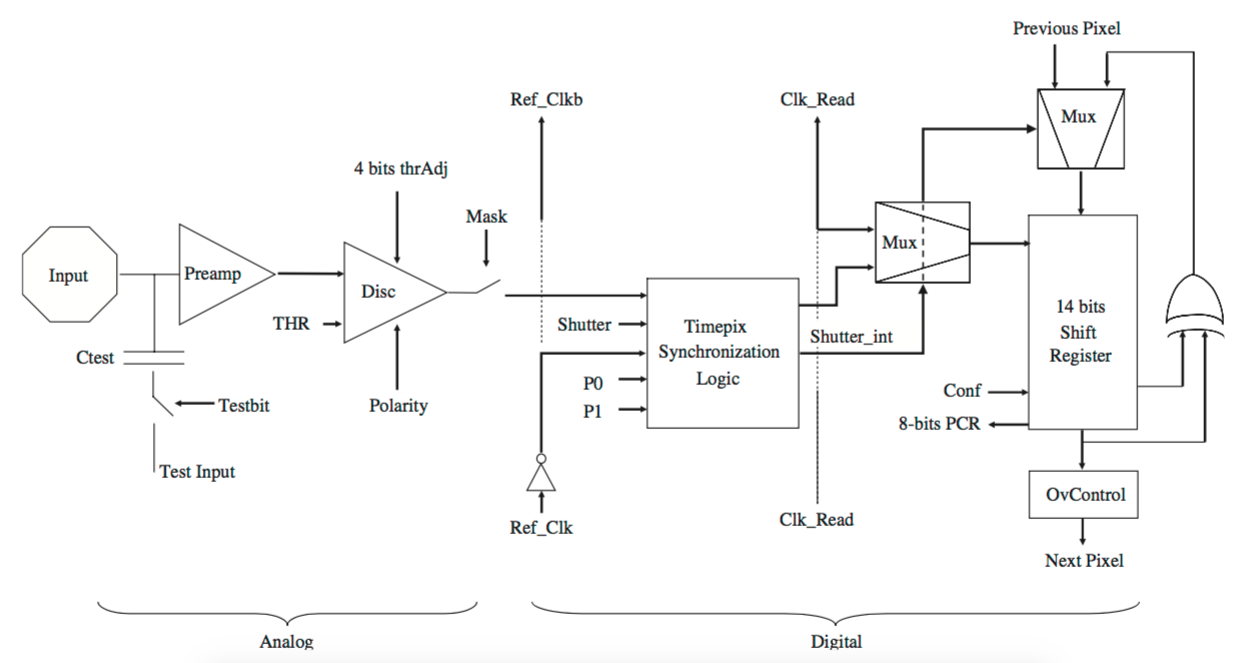
\includegraphics[width=\textwidth]{./figures/Calibration/Timepix_pixel_cell_schematic.jpg}
  \caption{Timepix pixel cell schematic. From ~\cite{art:tmpx}.}
  \label{fig:Timepix_pixel_cell_schematic}
\end{figure}

\subsection{Threshold equalisation} \label{sec:ThresholdEqualisation}
In semiconductor electronics, manufacturing imperfections cause
variations in the performance within the device. The threshold is one
of the most affected parameters and its global value set can vary
highly from one pixel to another within the pixel matrix. For the same
threshold value, the voltage on the discriminator can vary highly from
one pixel to another. To overcome this dispersion, a 4-bit local
threshold adjustment is applied to each pixel in order to make a
uniform global threshold. The photon counting mode is then
employed. The equalisation consists of adjusting this local threshold
by first setting its value to 0000. The global threshold DAC, THL, is
scanned and the number of pixels responding are counted. Then the
adjustment bit is set to 1111 and THL is scanned again. For each
pixel, the operation range is known. Assuming a linear relationship
between the two points, the adjustment threshold is adjusted in such a
way that the global threshold dispersion will remain uniform across
the matrix.


\section{Calibration} \label{sec:calibration}
\subsection{Energy and time
  calibration} \label{sec:TOT_TOA_calibration}
\begin{equation}
  \text{TOT} = a \, E + b - \frac{c}{E - t} \; ,
  \label{eq:TOTsurrogateFunction}
\end{equation}

\begin{figure}[htbp] \centering
  \begin{subfigure}[b]{0.45\textwidth}
    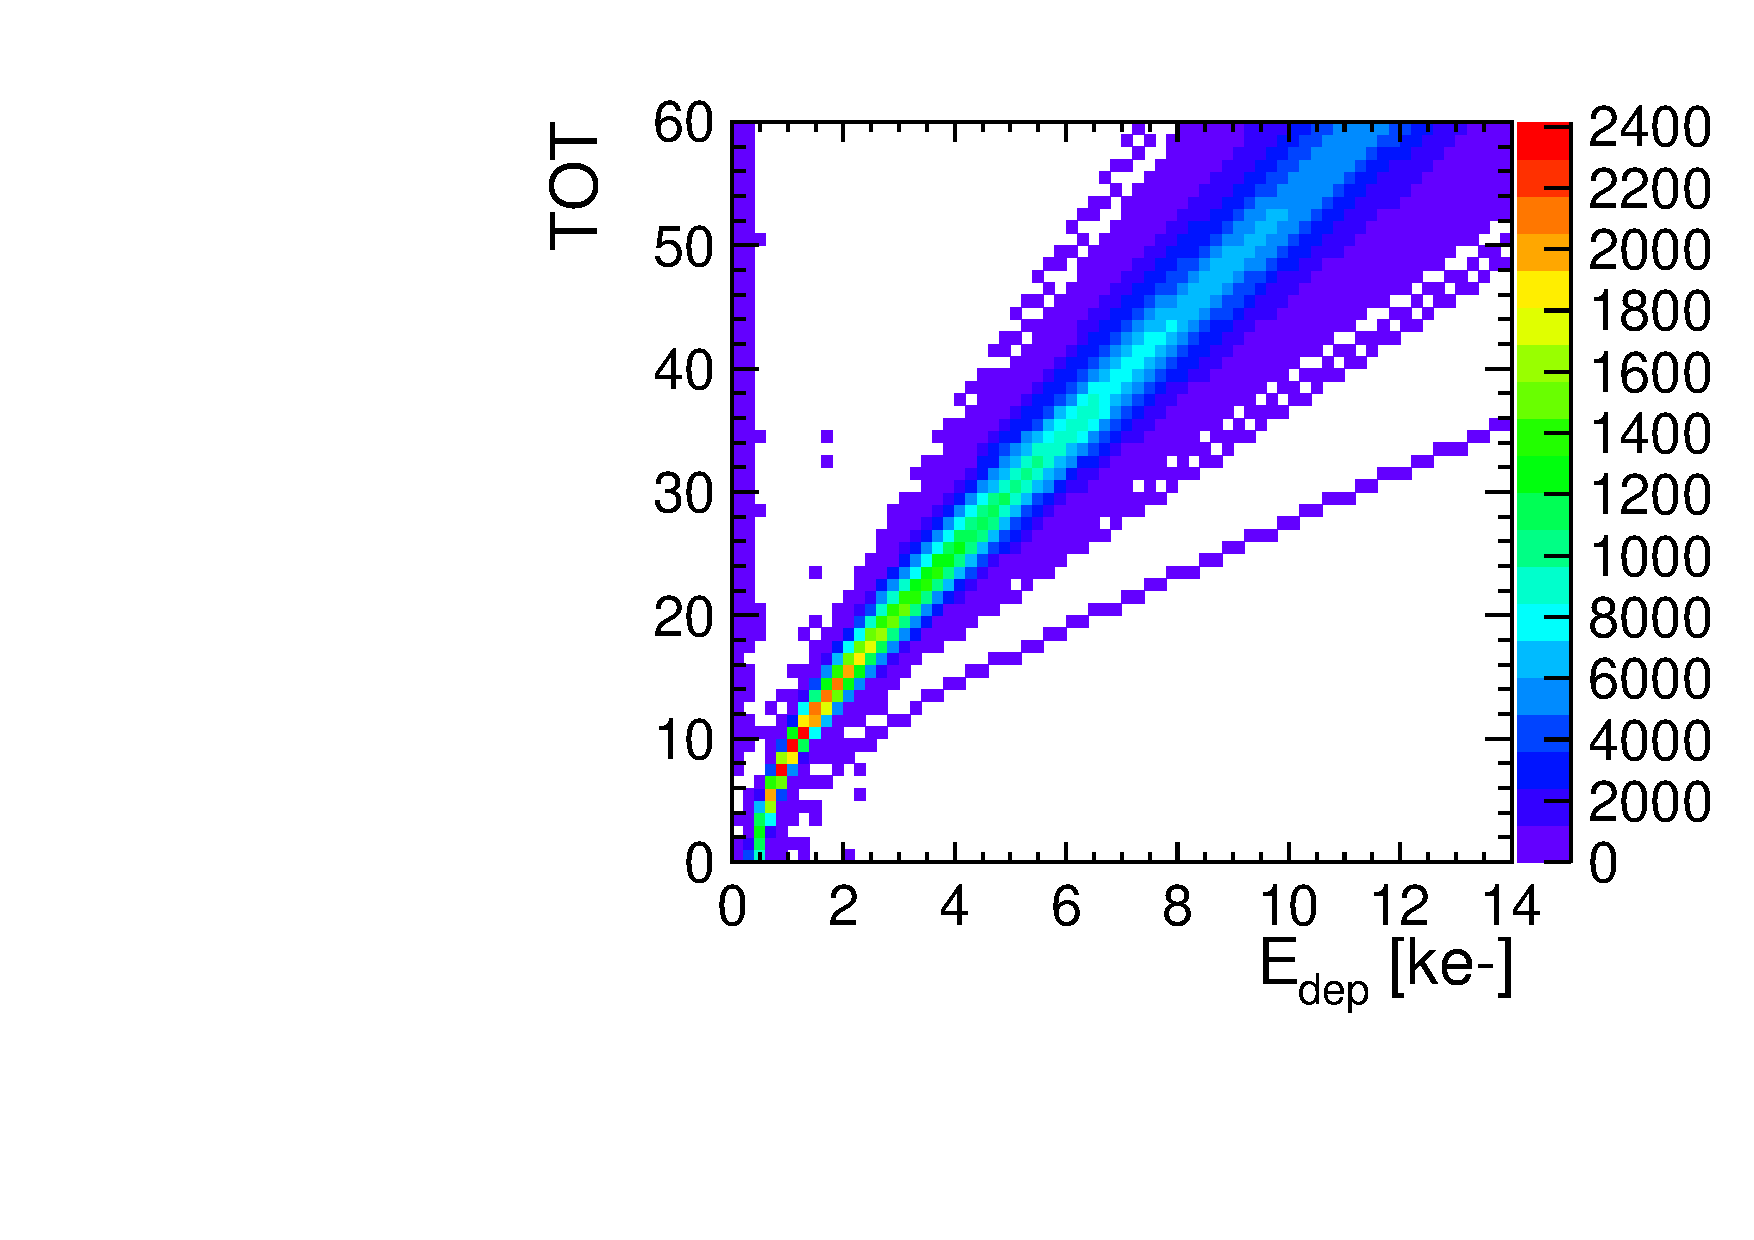
\includegraphics[width=\textwidth]{./figures/Calibration/TOTcalibration_W0005_E02_thresh1160.pdf}
    \caption{W5\_E2: THL=1160}
  \end{subfigure} \hfill
  \begin{subfigure}[b]{0.45\textwidth}
    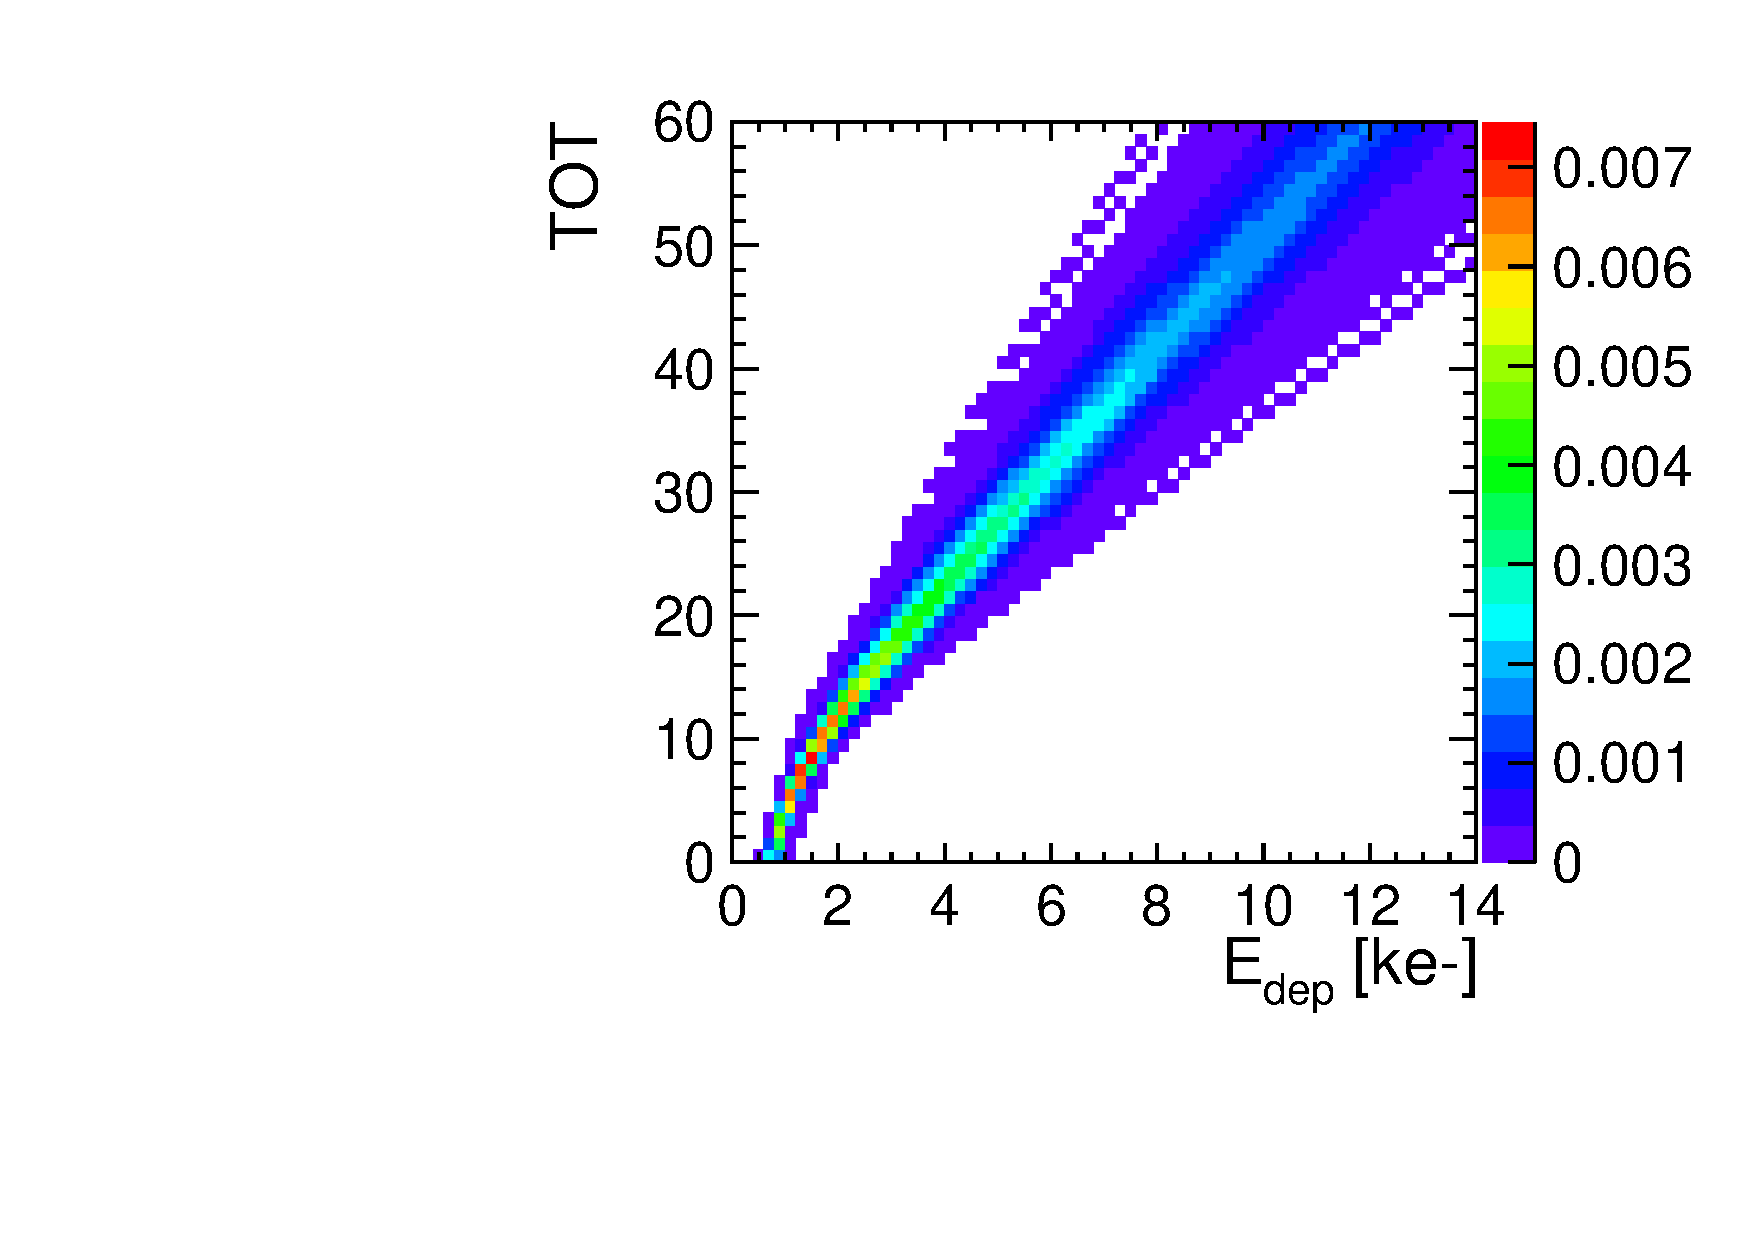
\includegraphics[width=\textwidth]{./figures/Calibration/TOTcalibration_W0005_E02_thresh1190.pdf}
    \caption{W5\_E2: THL=1190}
  \end{subfigure}
  \caption{TOT calibration for W5\_E2.}
  \label{fig:TOTcalibW5E2}
\end{figure}

\begin{figure}[htbp] \centering
  \begin{subfigure}[b]{0.45\textwidth}
    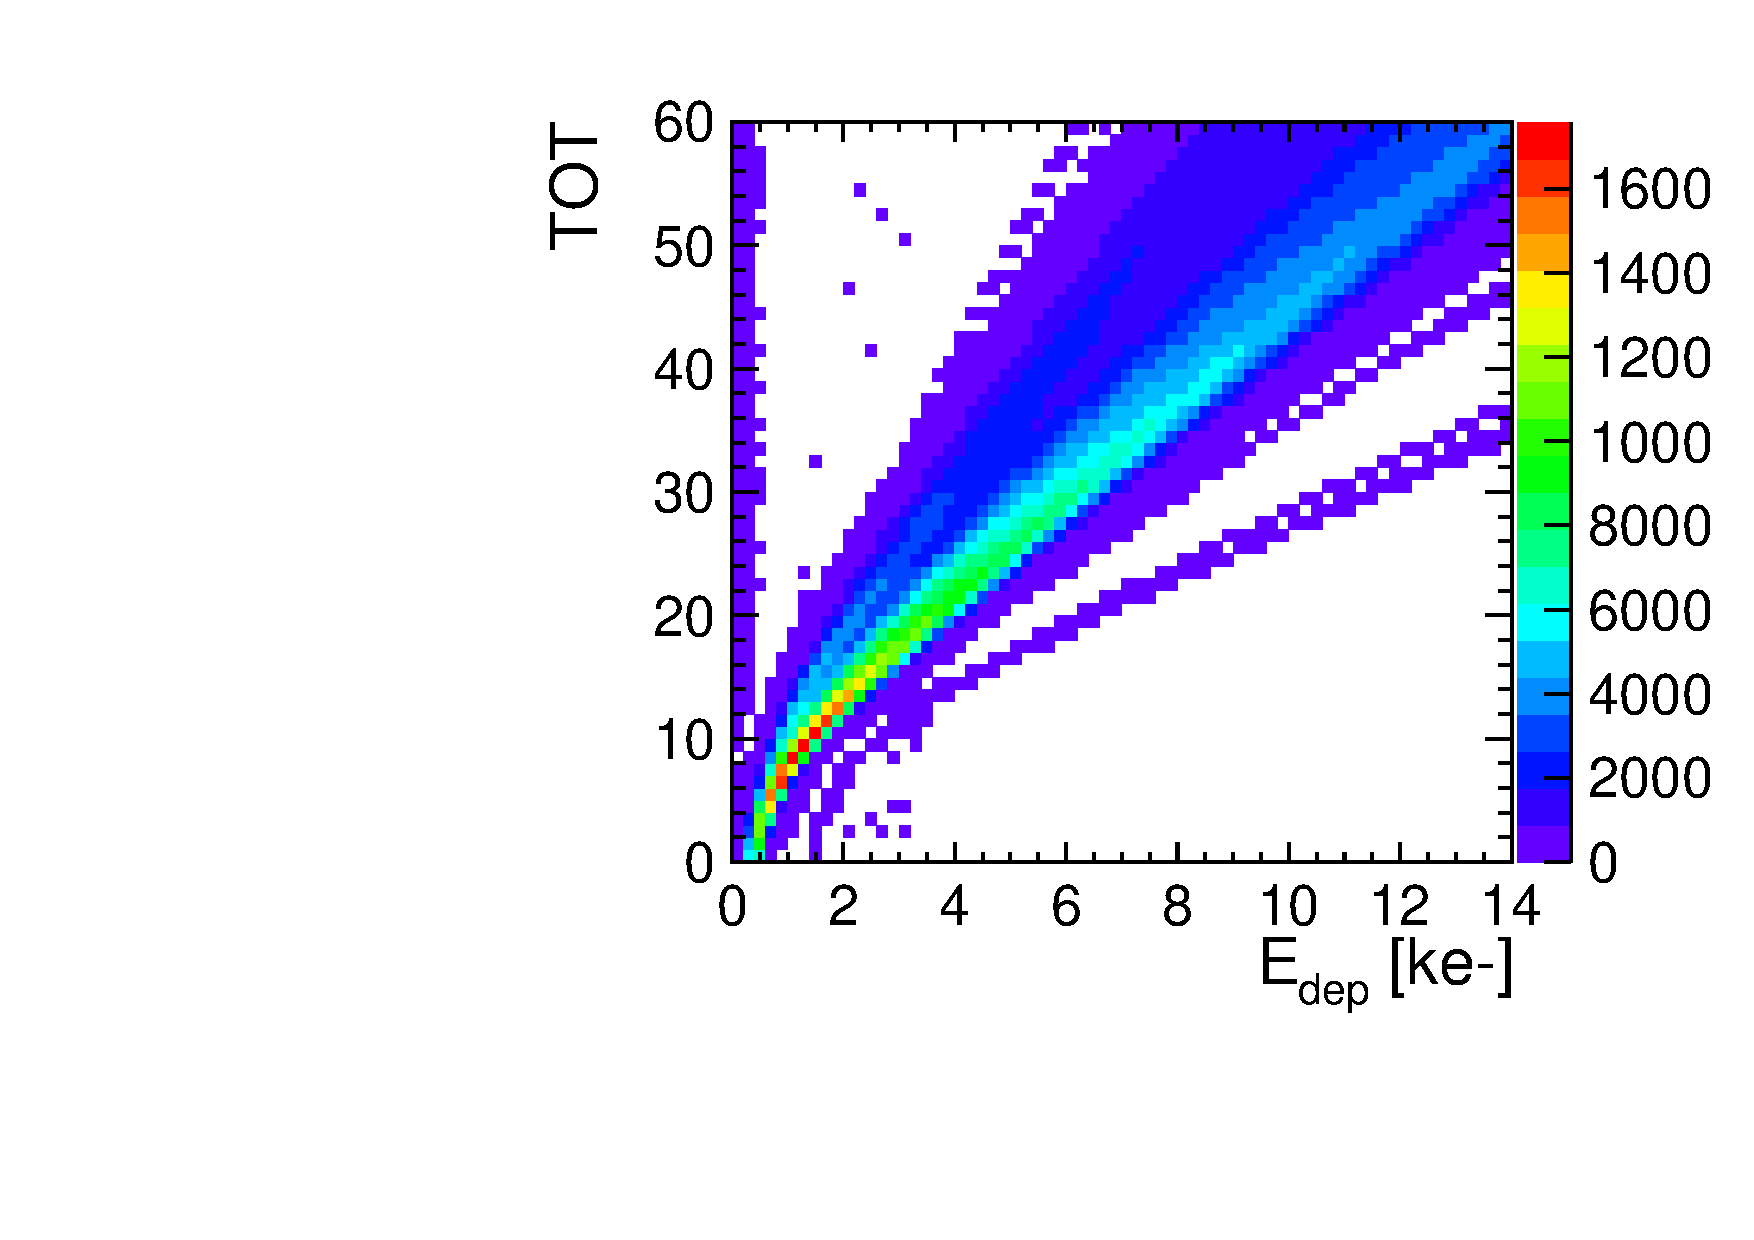
\includegraphics[width=\textwidth]{./figures/Calibration/TOTcalibration_W0005_F01_thresh1153.pdf}
    \caption{TOT calibration for W5\_F1, THL=1153.}
    \label{fig:TOTcalibW5F1}
  \end{subfigure}\hfill
  \begin{subfigure}[b]{0.45\textwidth}
    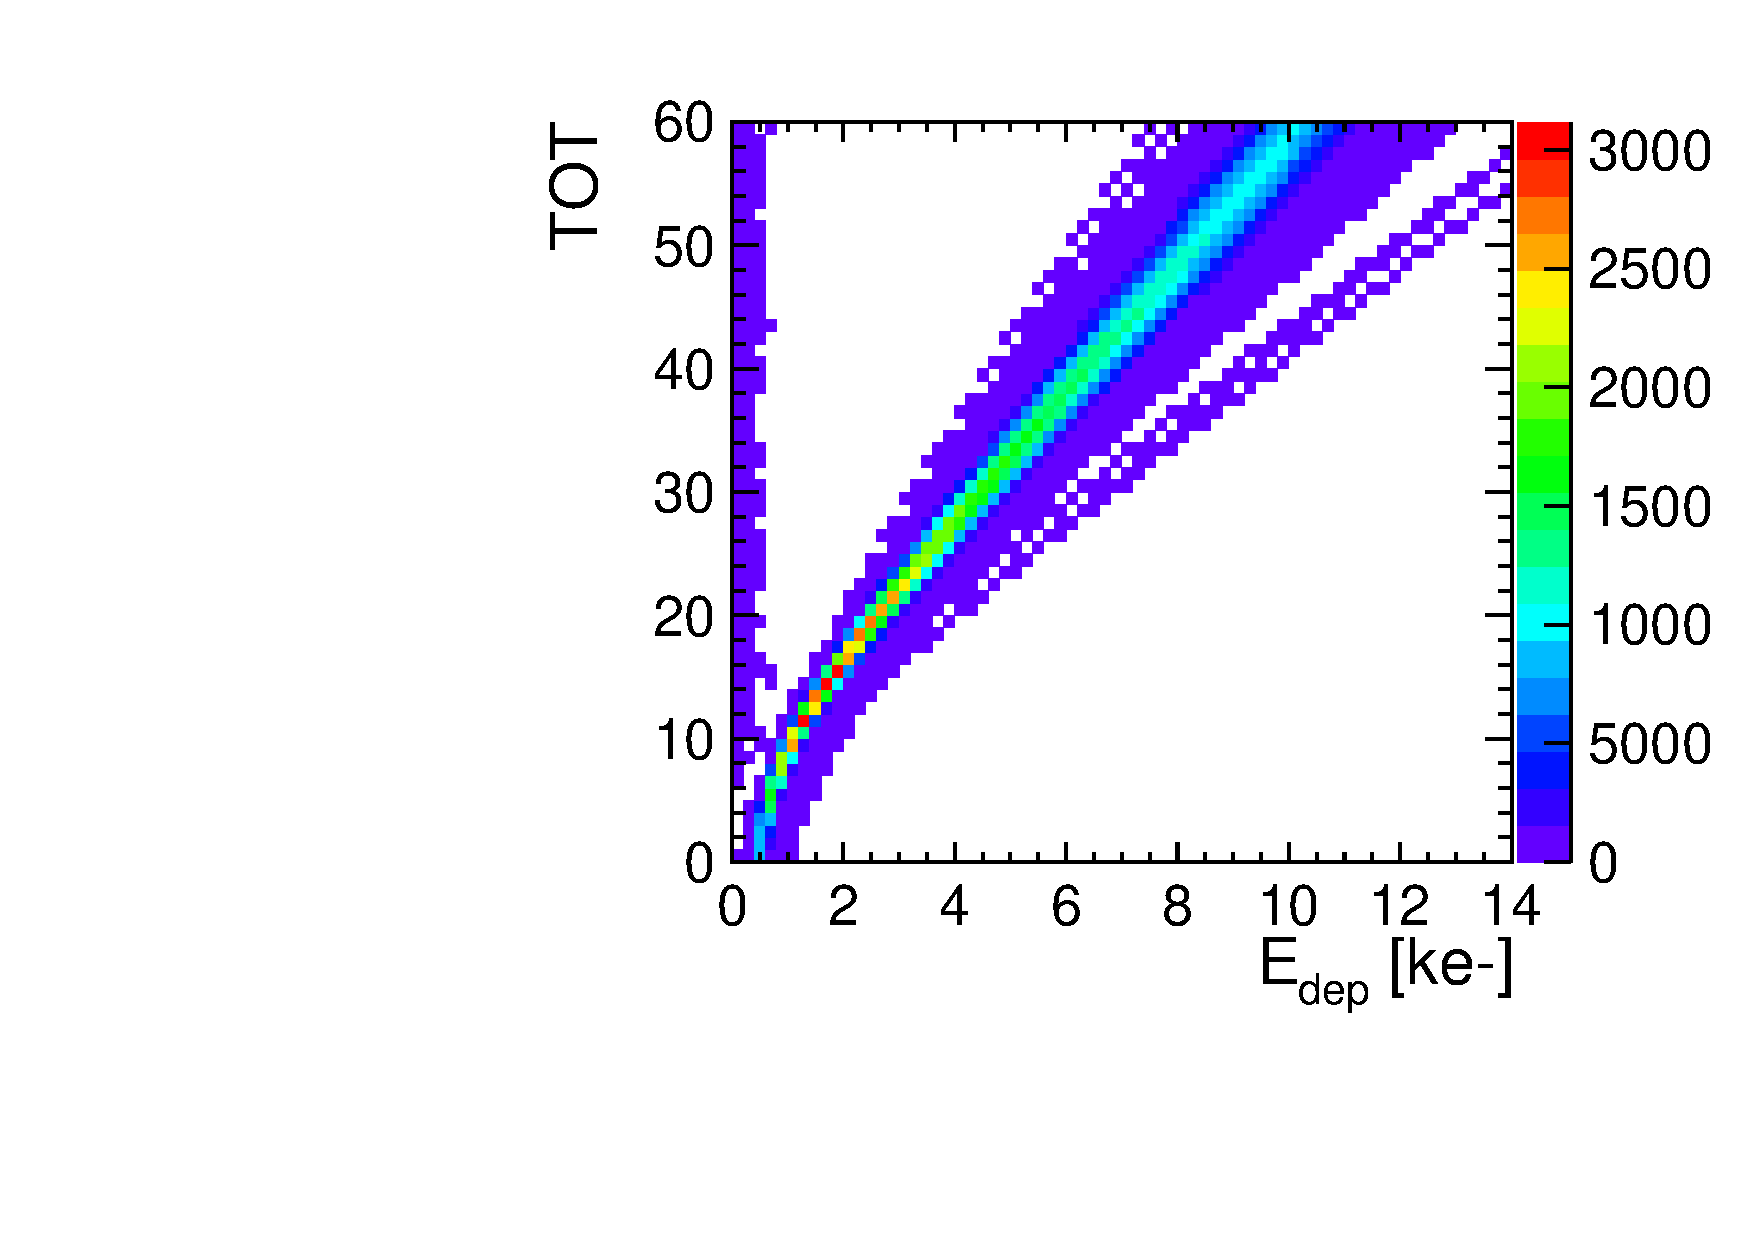
\includegraphics[width=\textwidth]{./figures/Calibration/TOTcalibration_W0019_C07_thresh1148.pdf}
    \caption{TOT calibration for W19\_C7, THL=1148.}
    \label{fig:TOTcalibW19C7}
  \end{subfigure}
\end{figure}


\begin{figure}[htbp] \centering
  \begin{subfigure}[b]{0.45\textwidth}
    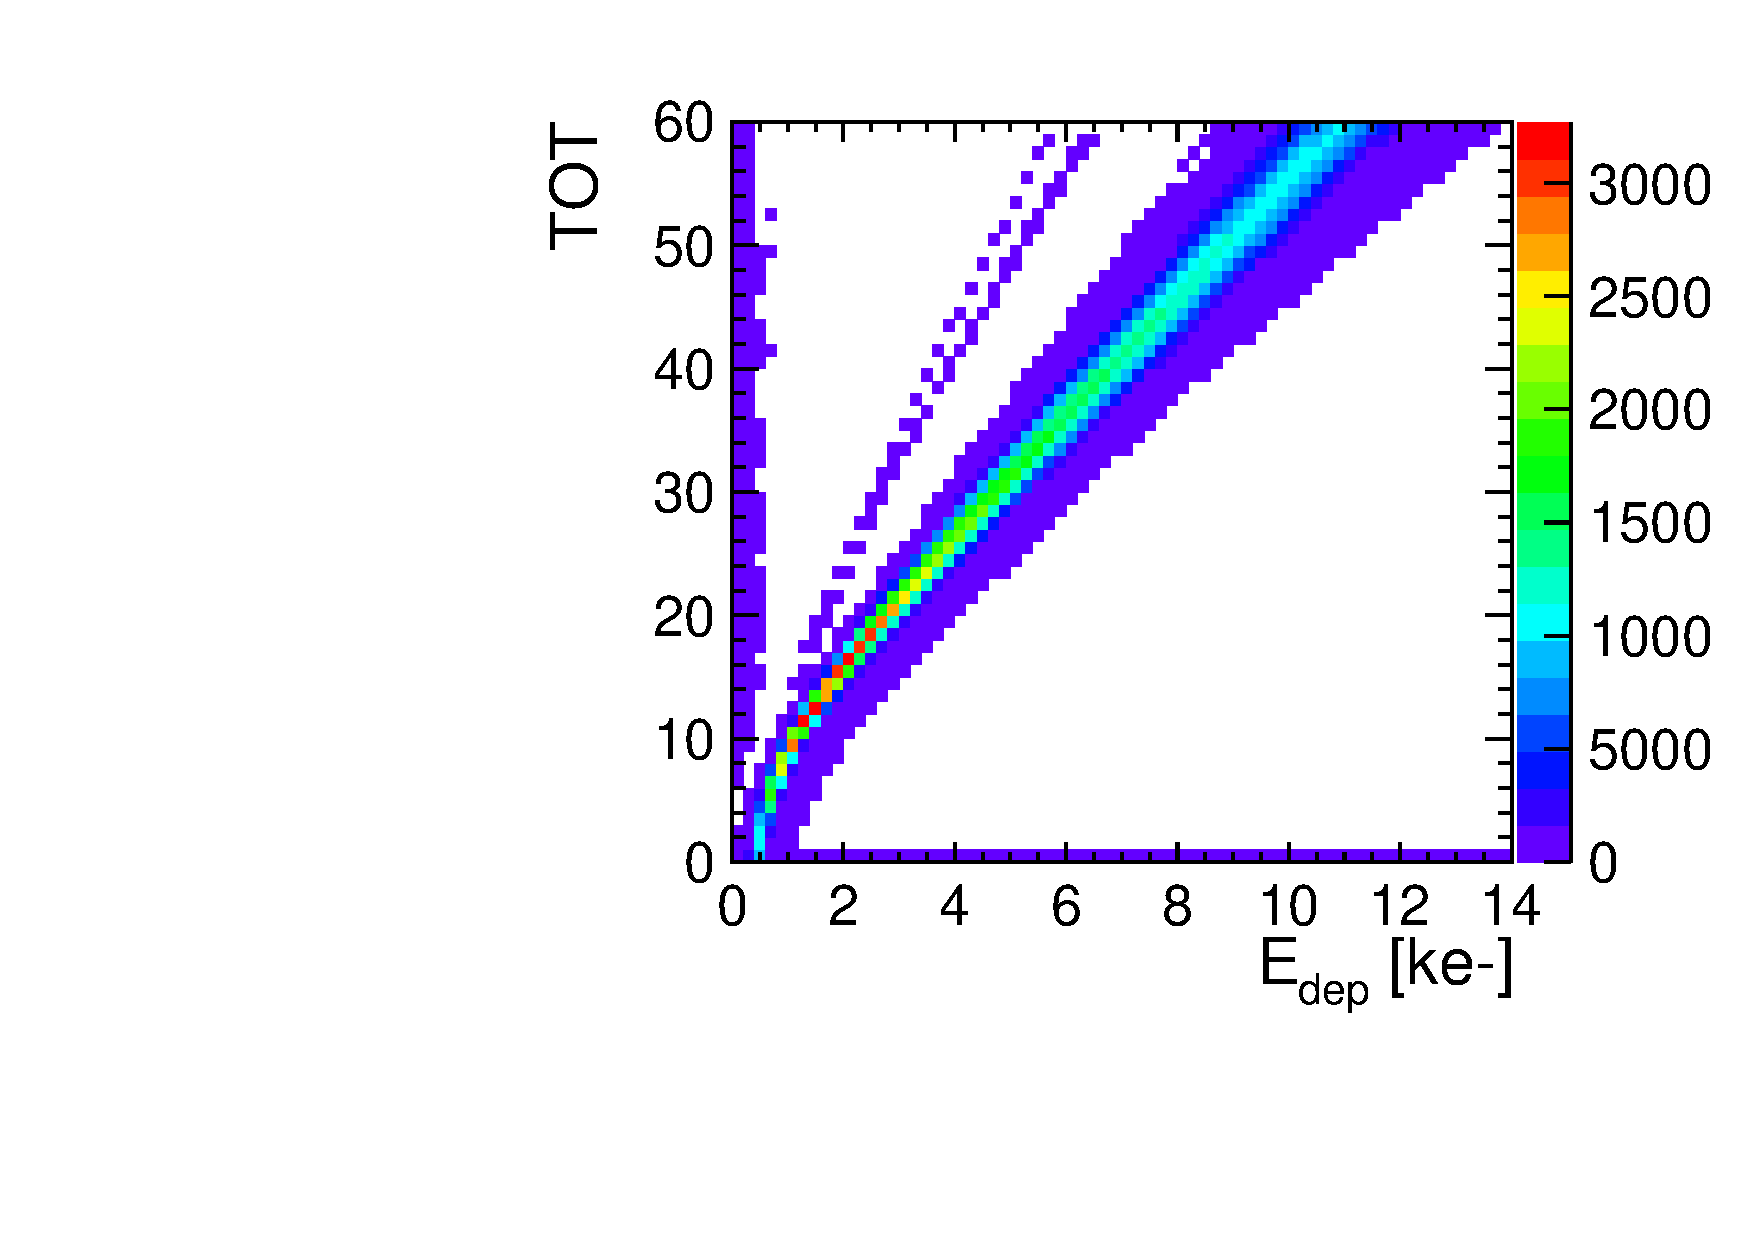
\includegraphics[width=\textwidth]{./figures/Calibration/TOTcalibration_W0019_G07_thresh1190.pdf}
    \caption{TOT calibration for W19\_G7, THL=1190.}
    \label{fig:TOTcalibW19G7}
  \end{subfigure}\hfill
  \begin{subfigure}[b]{0.45\textwidth}
    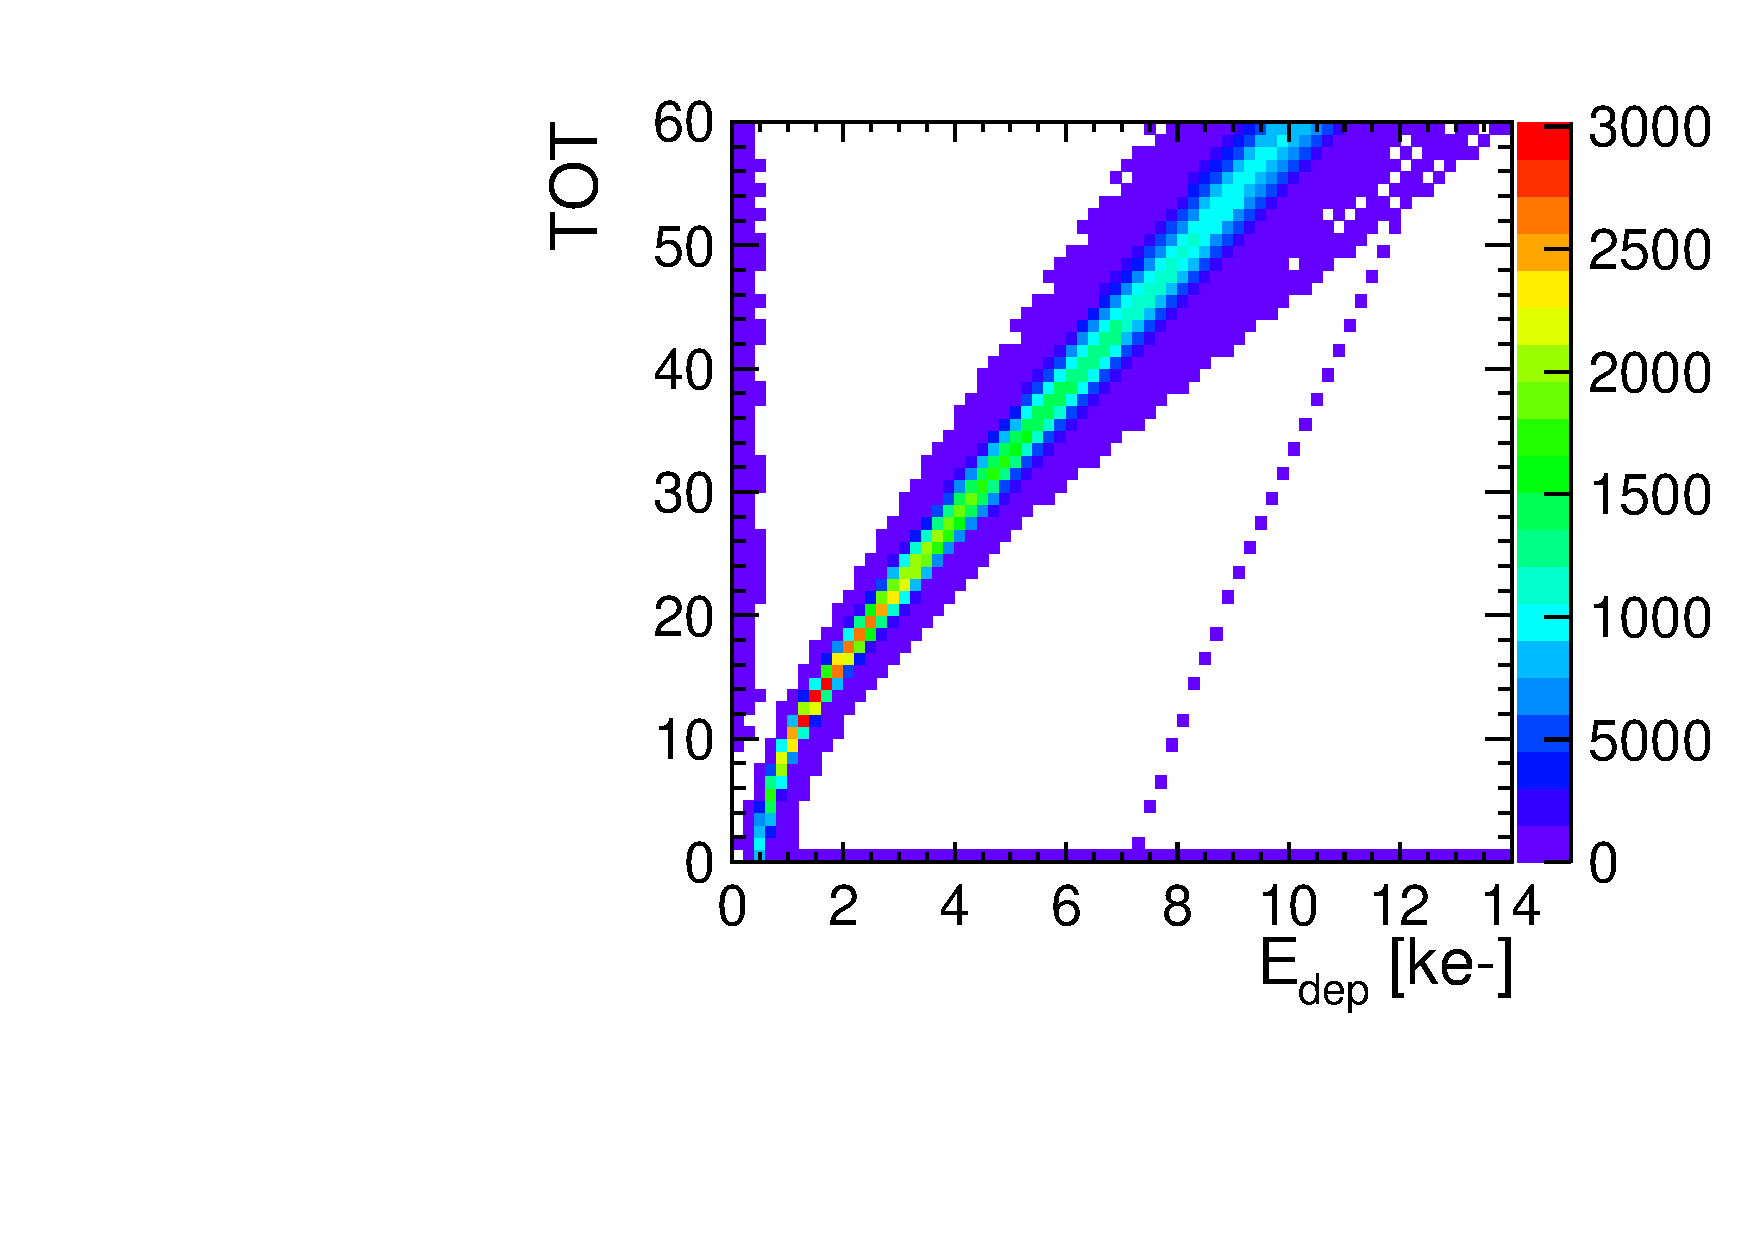
\includegraphics[width=\textwidth]{./figures/Calibration/TOTcalibration_W0019_L08_thresh1133.pdf}
    \caption{TOT calibration for W19\_L8, THL=1133.}
    \label{fig:TOTcalibW19L8}
  \end{subfigure}
\end{figure}


\begin{figure}[htbp] \centering
  \begin{subfigure}[b]{0.45\textwidth}
    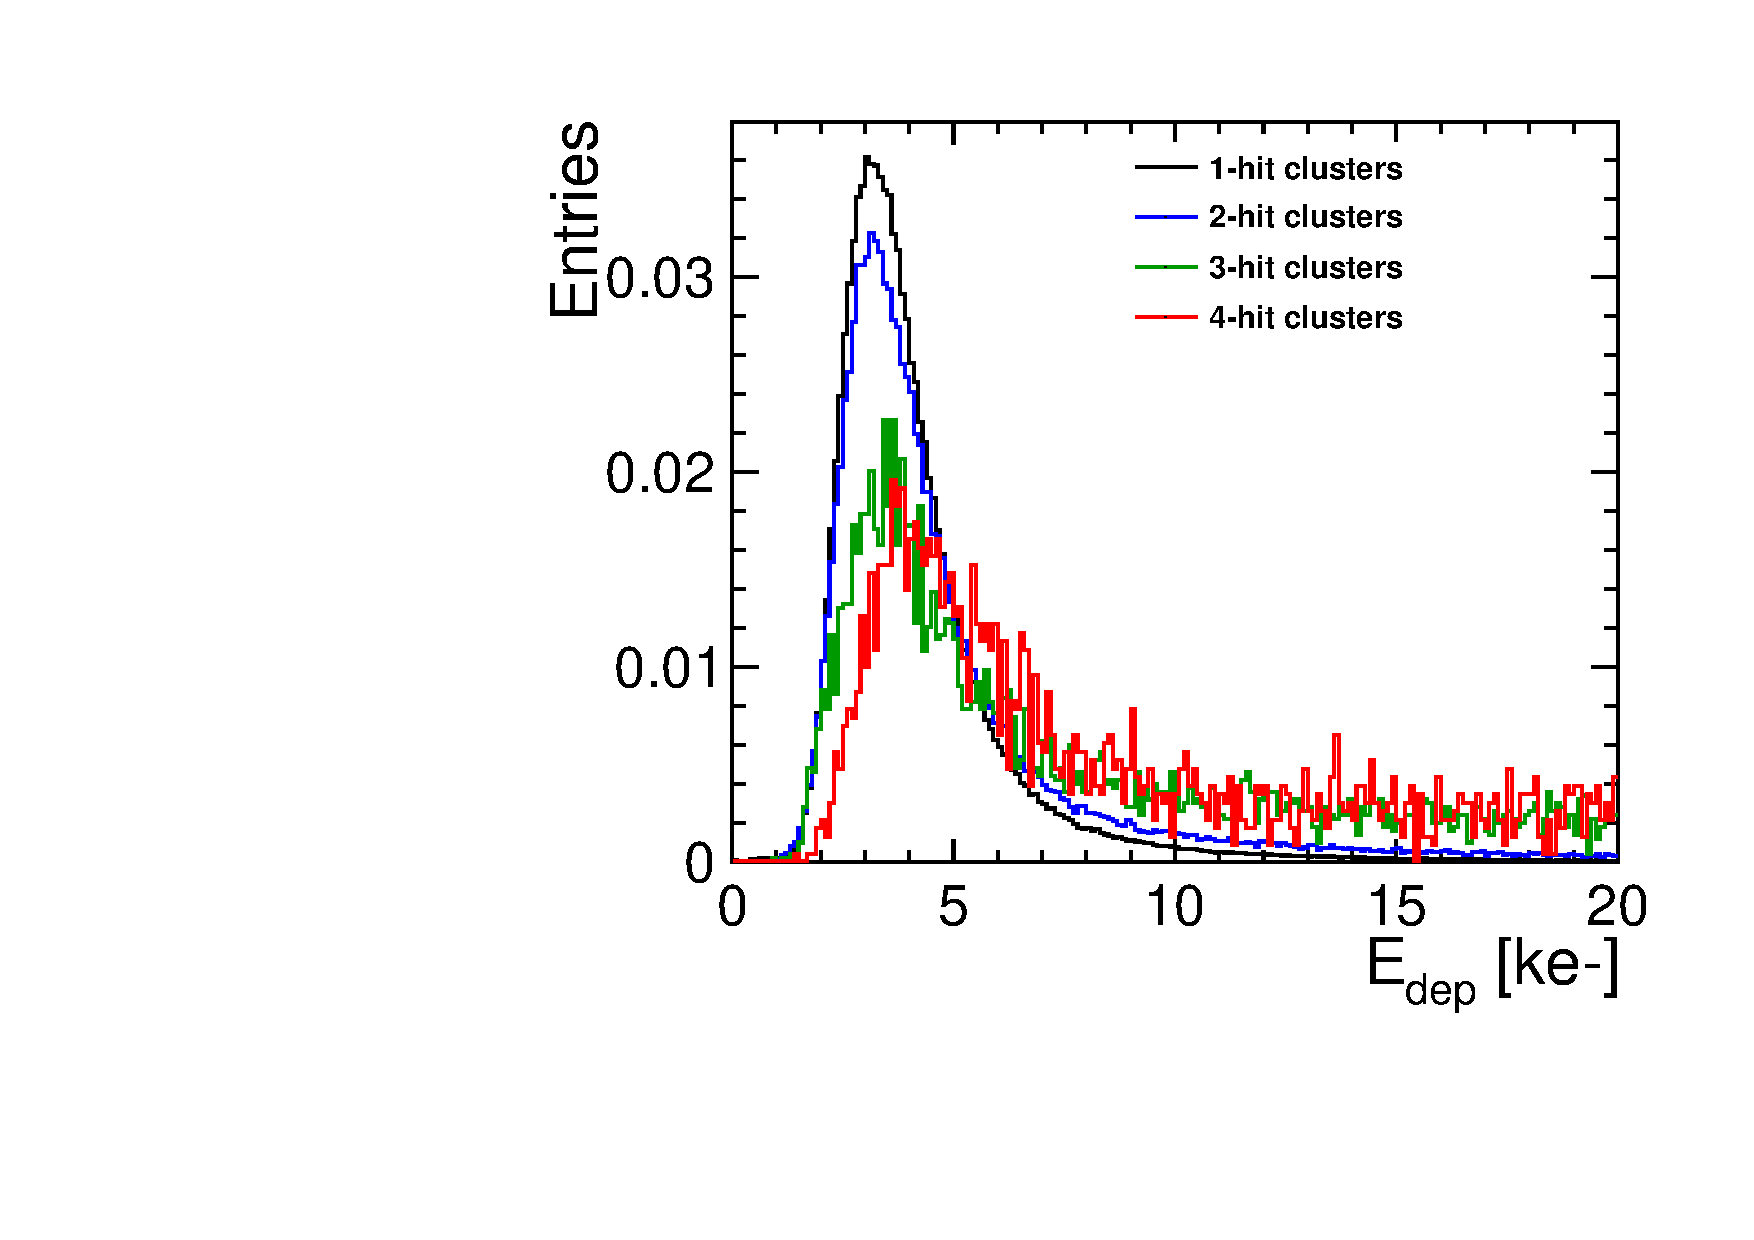
\includegraphics[width=\textwidth]{./figures/Calibration/Edep_Clusters_W0019_C07.pdf}
    \caption{}
  \end{subfigure}\hfill
  \begin{subfigure}[b]{0.45\textwidth}
    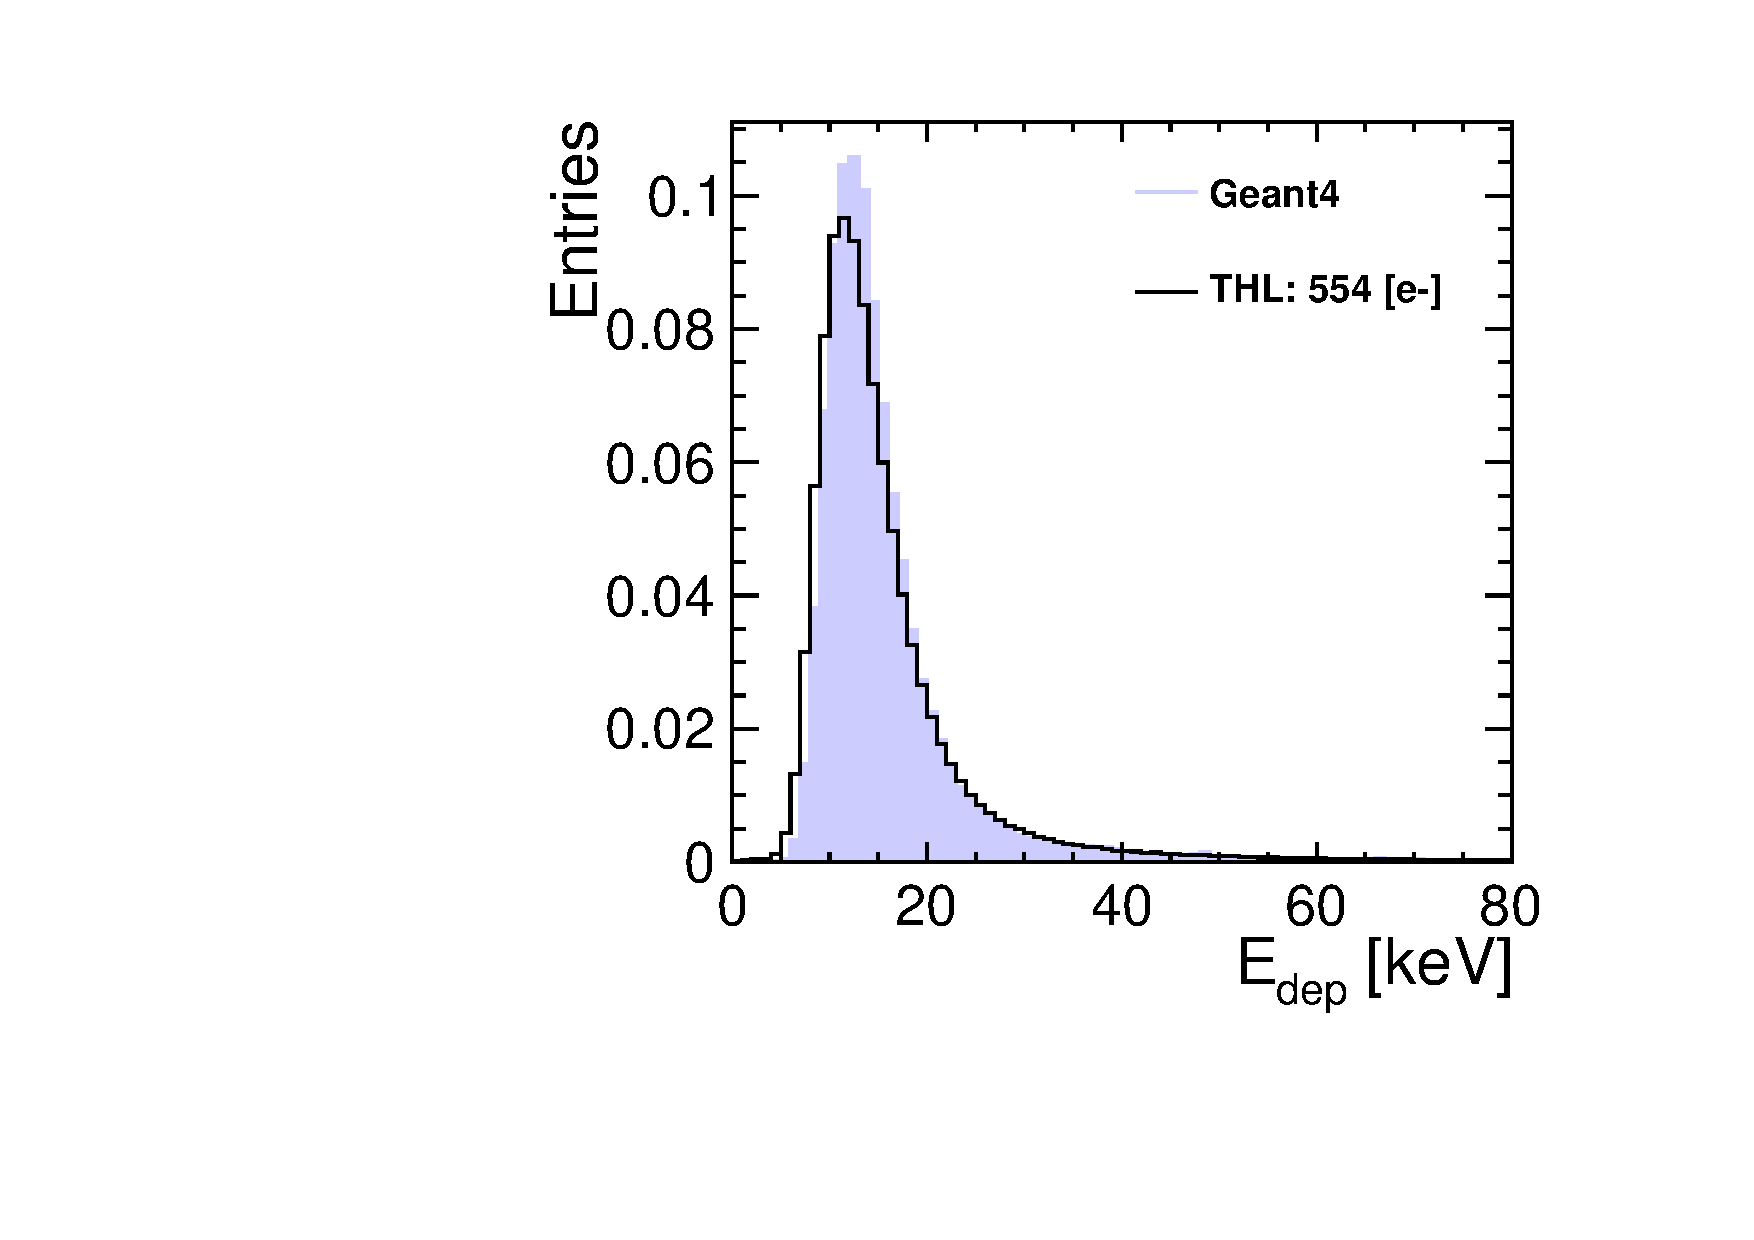
\includegraphics[width=\textwidth]{./figures/Calibration/Edep_G4_W0019_C07.pdf}
    \caption{}
  \end{subfigure}
  \caption{Energy deposition and comparison to
    \textsc{Geant4}. W0019\_C07, Run 902, THL=1148.}
  \label{fig:EdepW19C7}
\end{figure}


\begin{figure}[htbp] \centering
  \begin{subfigure}[b]{0.45\textwidth}
    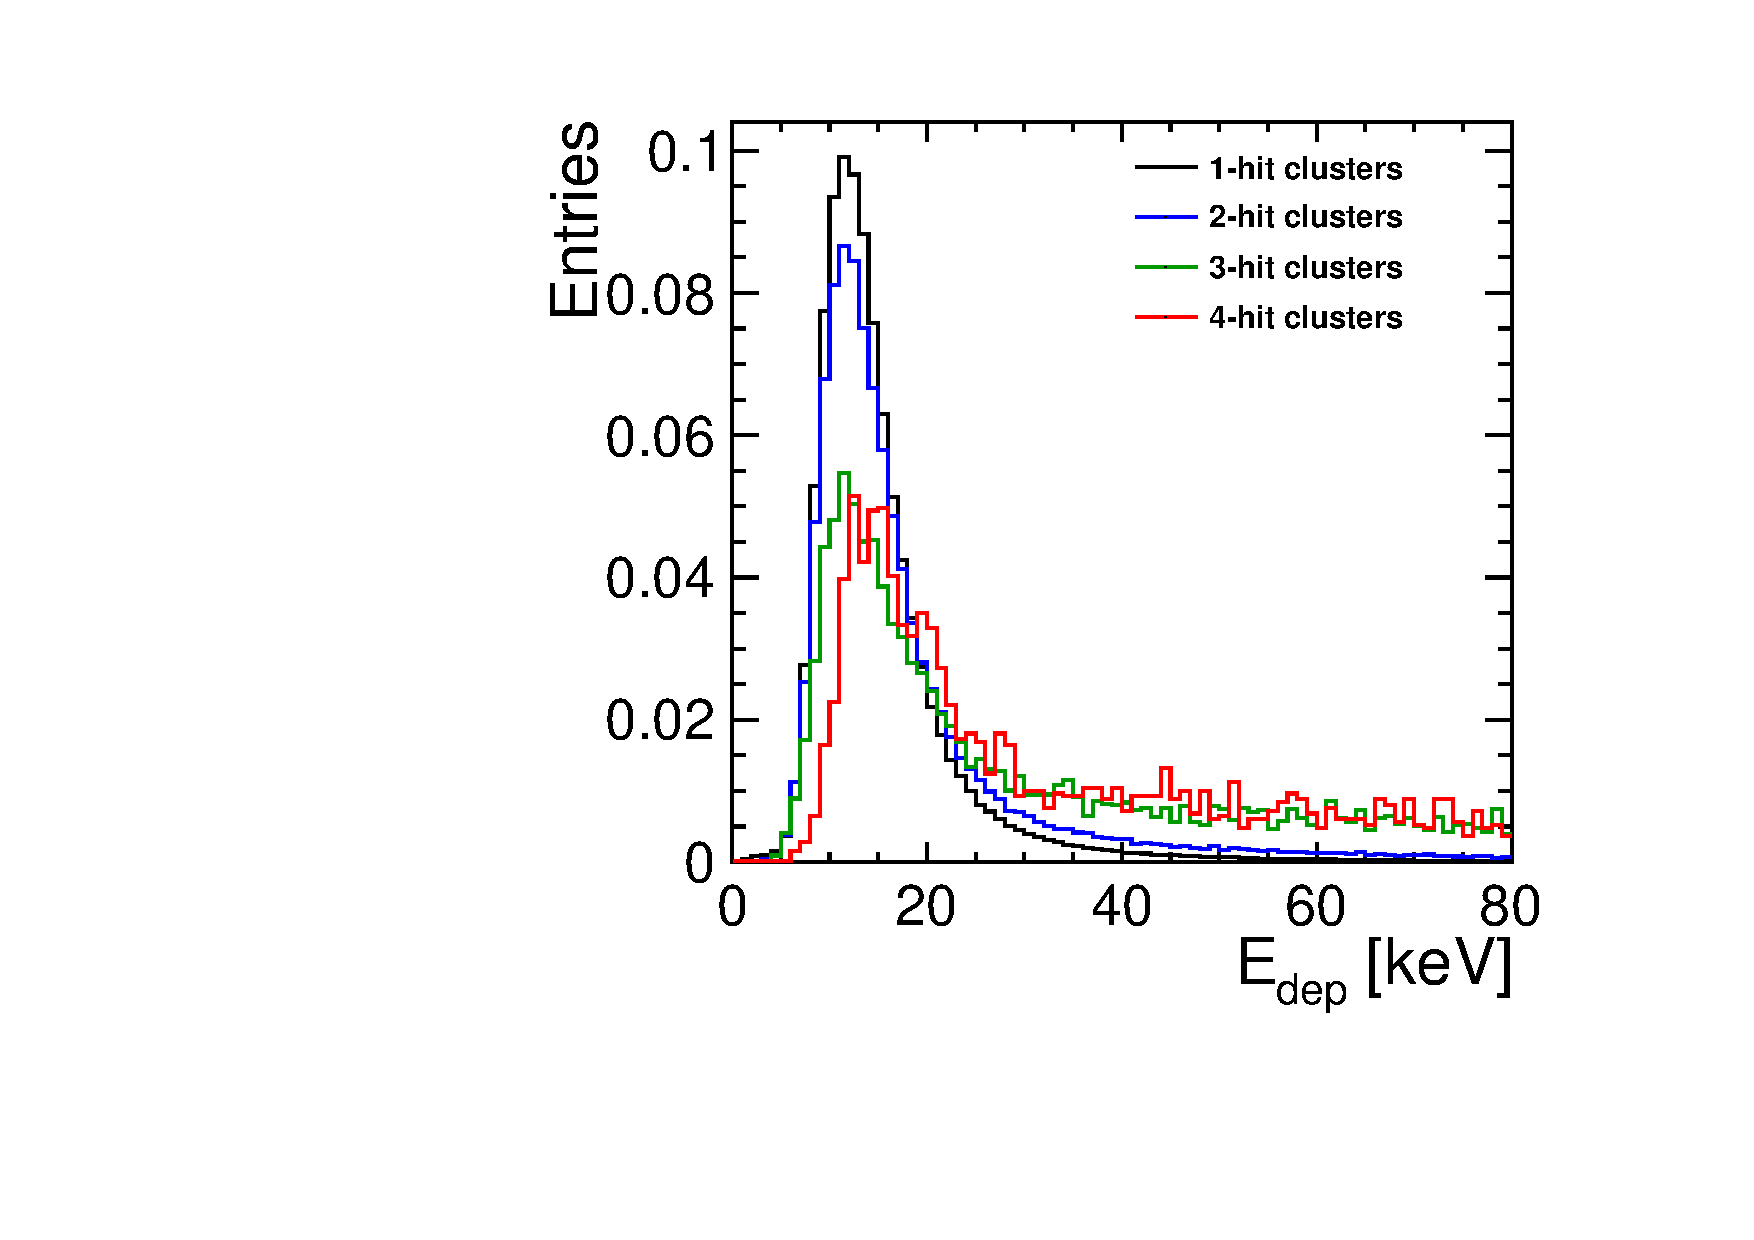
\includegraphics[width=\textwidth]{./figures/Calibration/Edep_Clusters_W0019_L08.pdf}
    \caption{}
  \end{subfigure}\hfill
  \begin{subfigure}[b]{0.45\textwidth}
    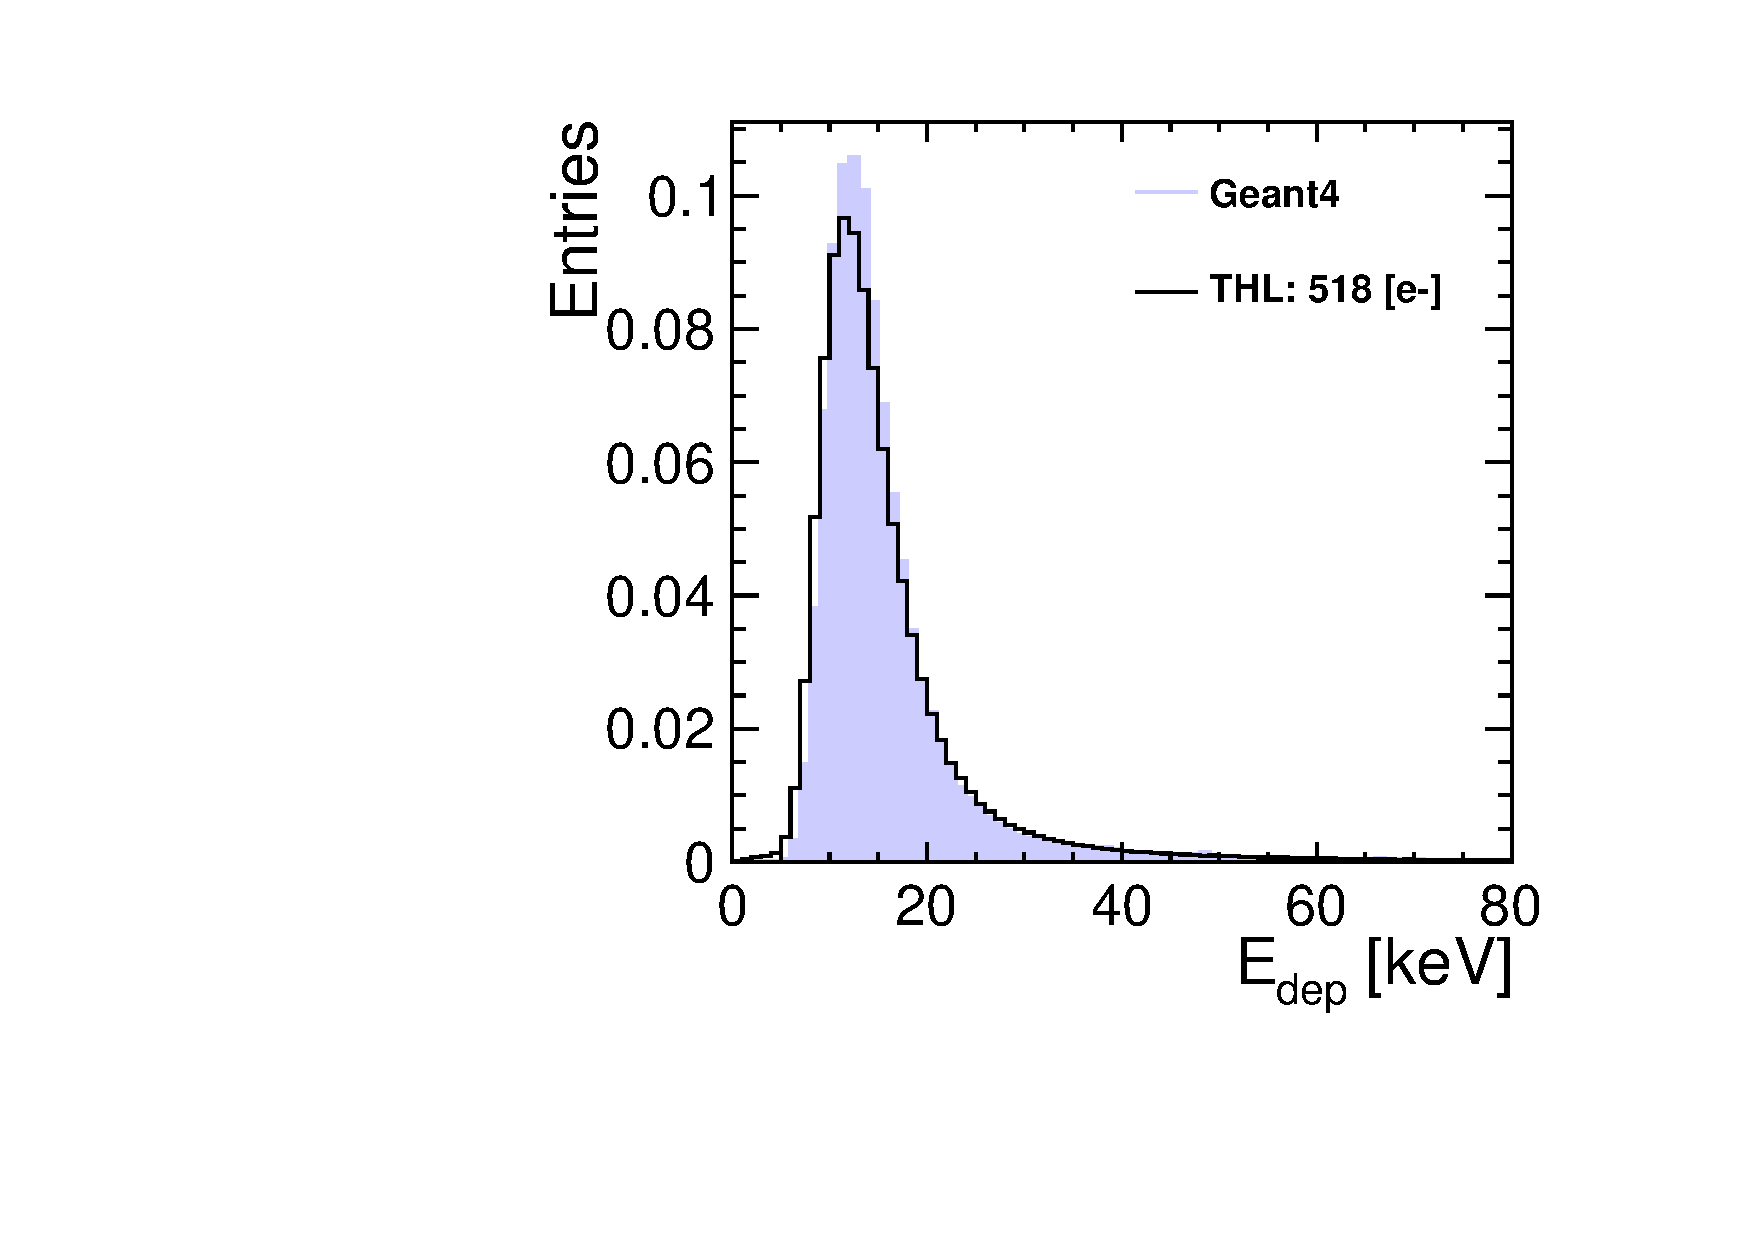
\includegraphics[width=\textwidth]{./figures/Calibration/Edep_G4_W0019_L08.pdf}
    \caption{}
  \end{subfigure}
  \caption{Energy deposition and comparison to
    \textsc{Geant4}. W0019\_L08, Run 1130, THL=1133.}
  \label{fig:EdepW19L8}
\end{figure}


\begin{figure}[htbp] \centering
  \begin{subfigure}[b]{0.45\textwidth}
    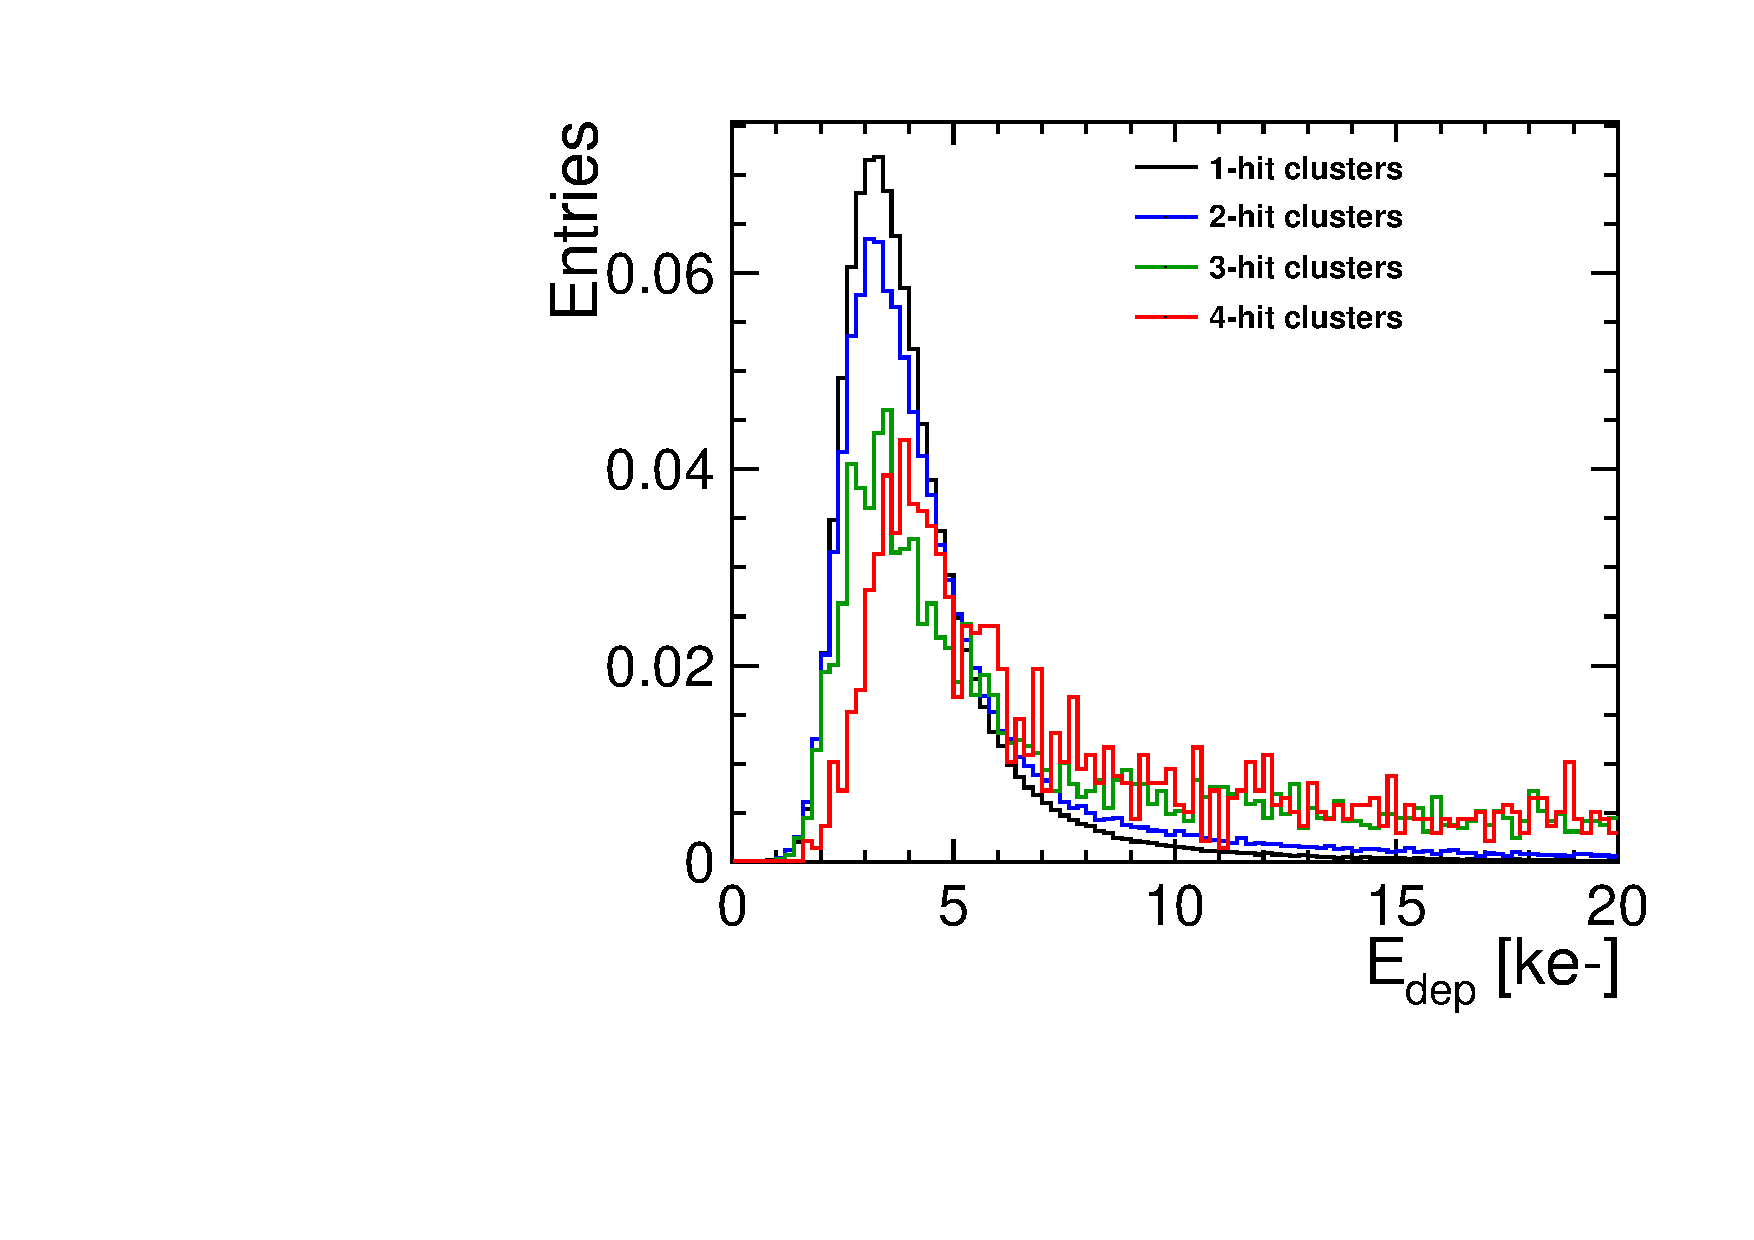
\includegraphics[width=\textwidth]{./figures/Calibration/Edep_Clusters_W0019_G07.pdf}
    \caption{}
  \end{subfigure}\hfill
  \begin{subfigure}[b]{0.45\textwidth}
    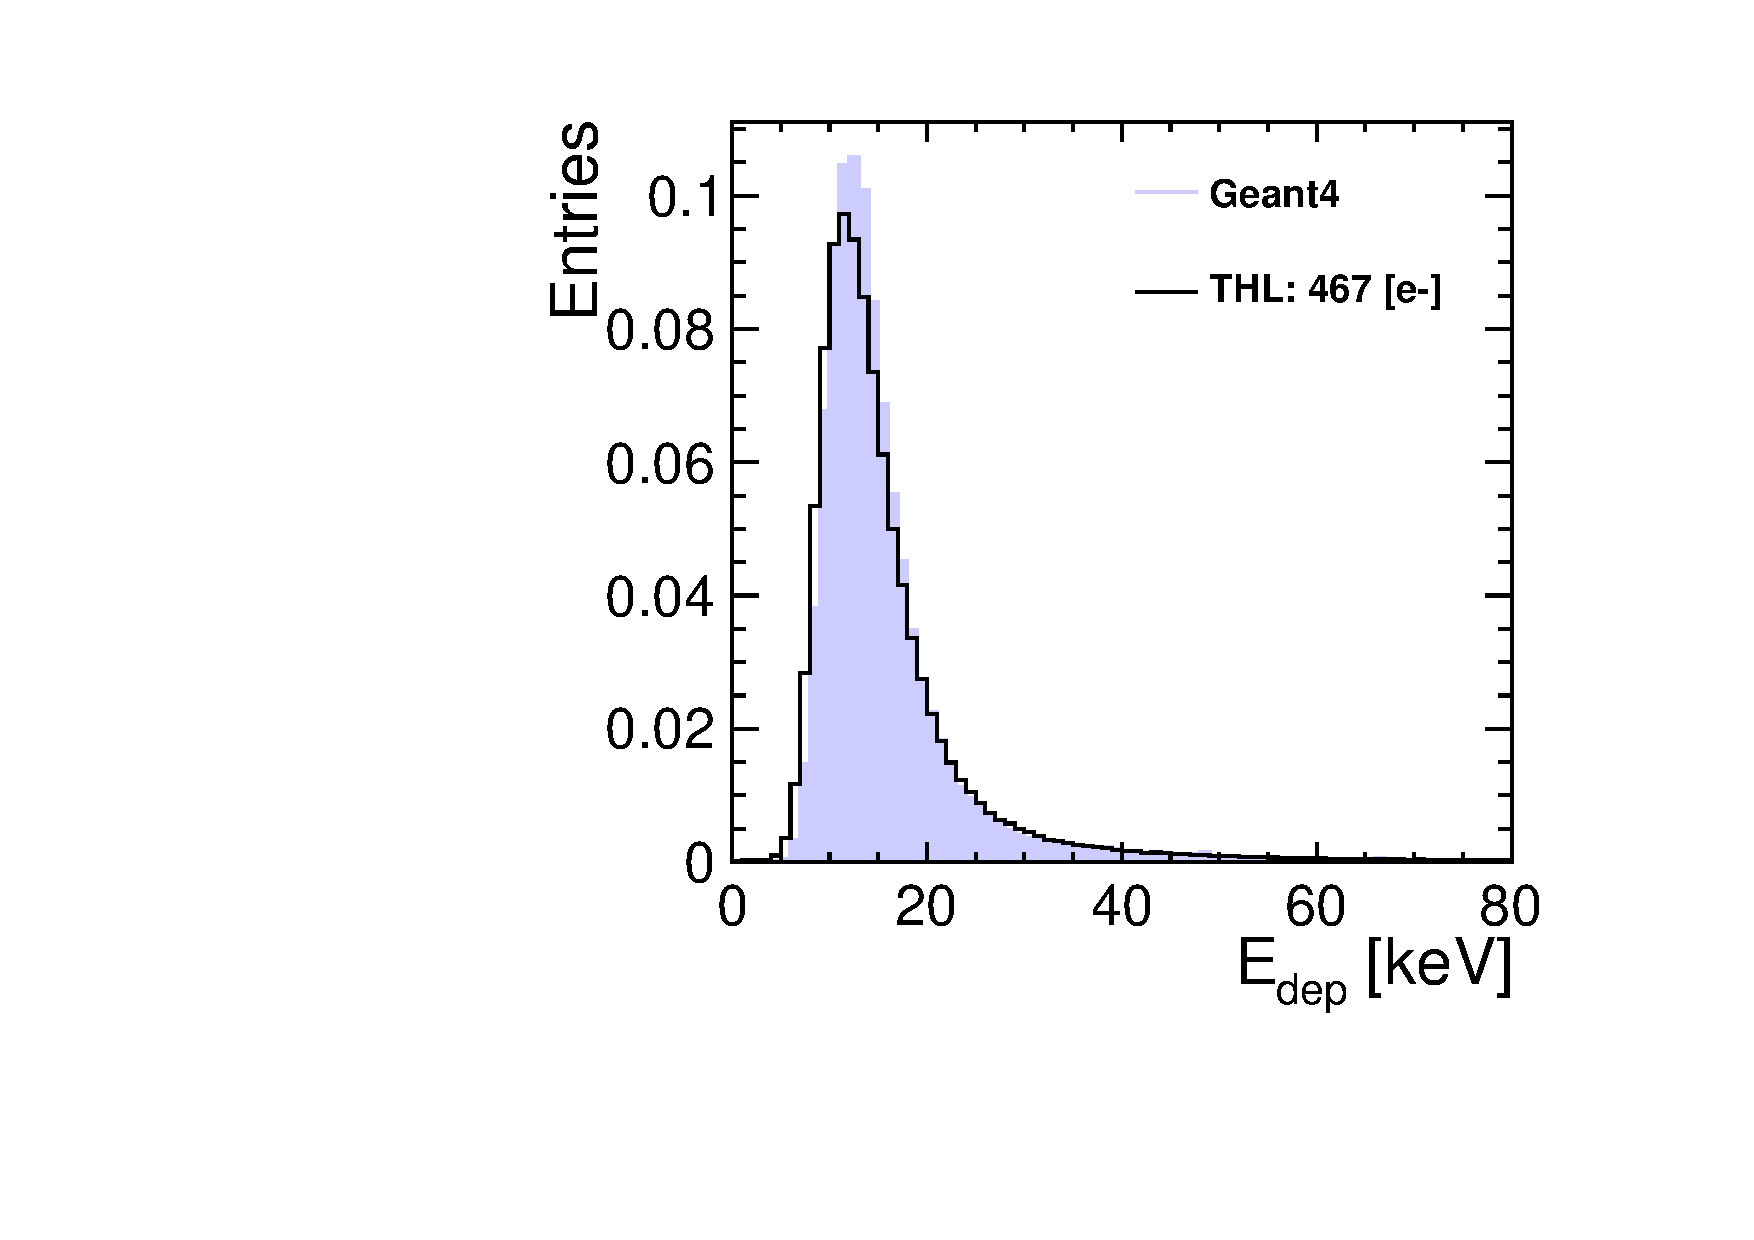
\includegraphics[width=\textwidth]{./figures/Calibration/Edep_G4_W0019_G07.pdf}
    \caption{}
  \end{subfigure}
  \caption{Energy deposition and comparison to
    \textsc{Geant4}. W0019\_G07, Run 1190, THL=995.}
  \label{fig:EdepW19L8}
\end{figure}


\begin{figure}[htbp] \centering
  \begin{subfigure}[b]{0.45\textwidth}
    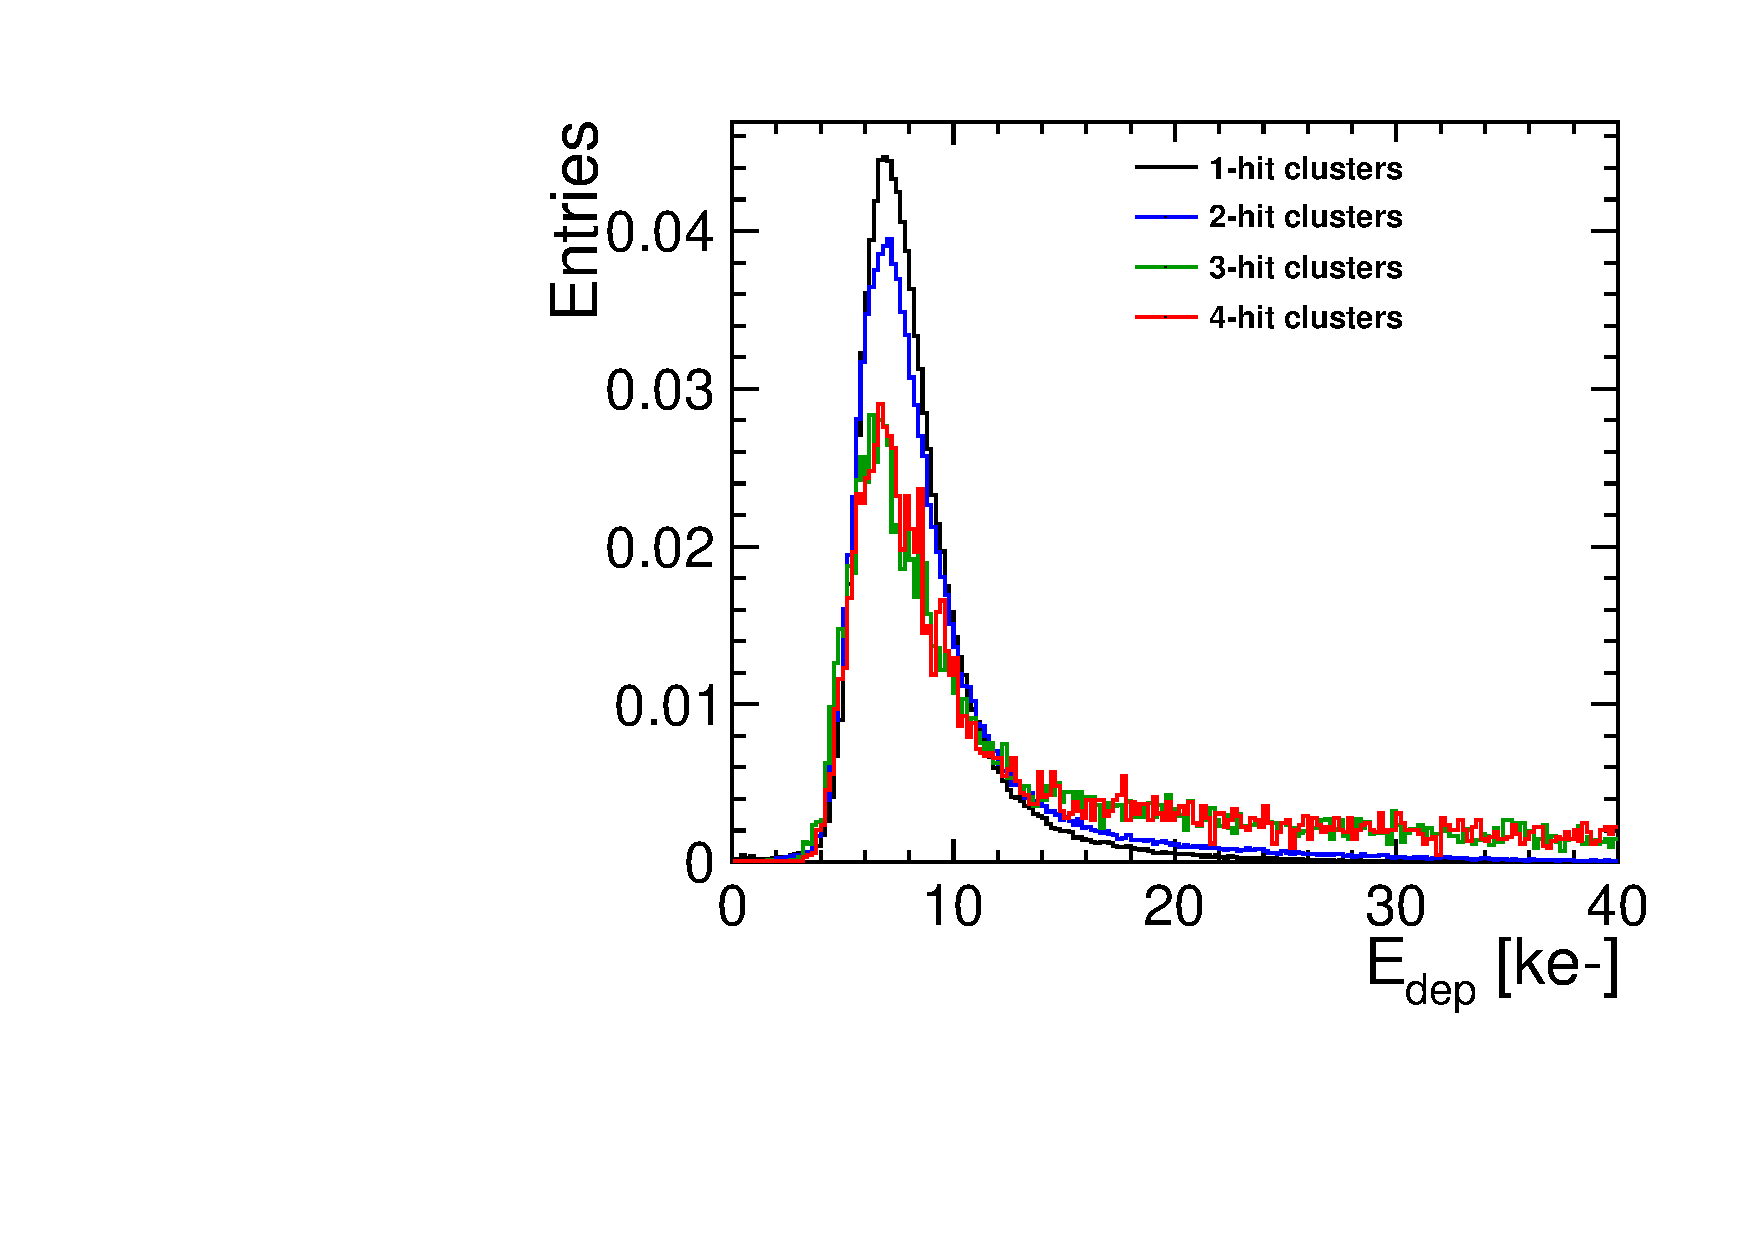
\includegraphics[width=\textwidth]{./figures/Calibration/Edep_Clusters_W0005_E02.pdf}
    \caption{}
  \end{subfigure}\hfill
  \begin{subfigure}[b]{0.45\textwidth}
    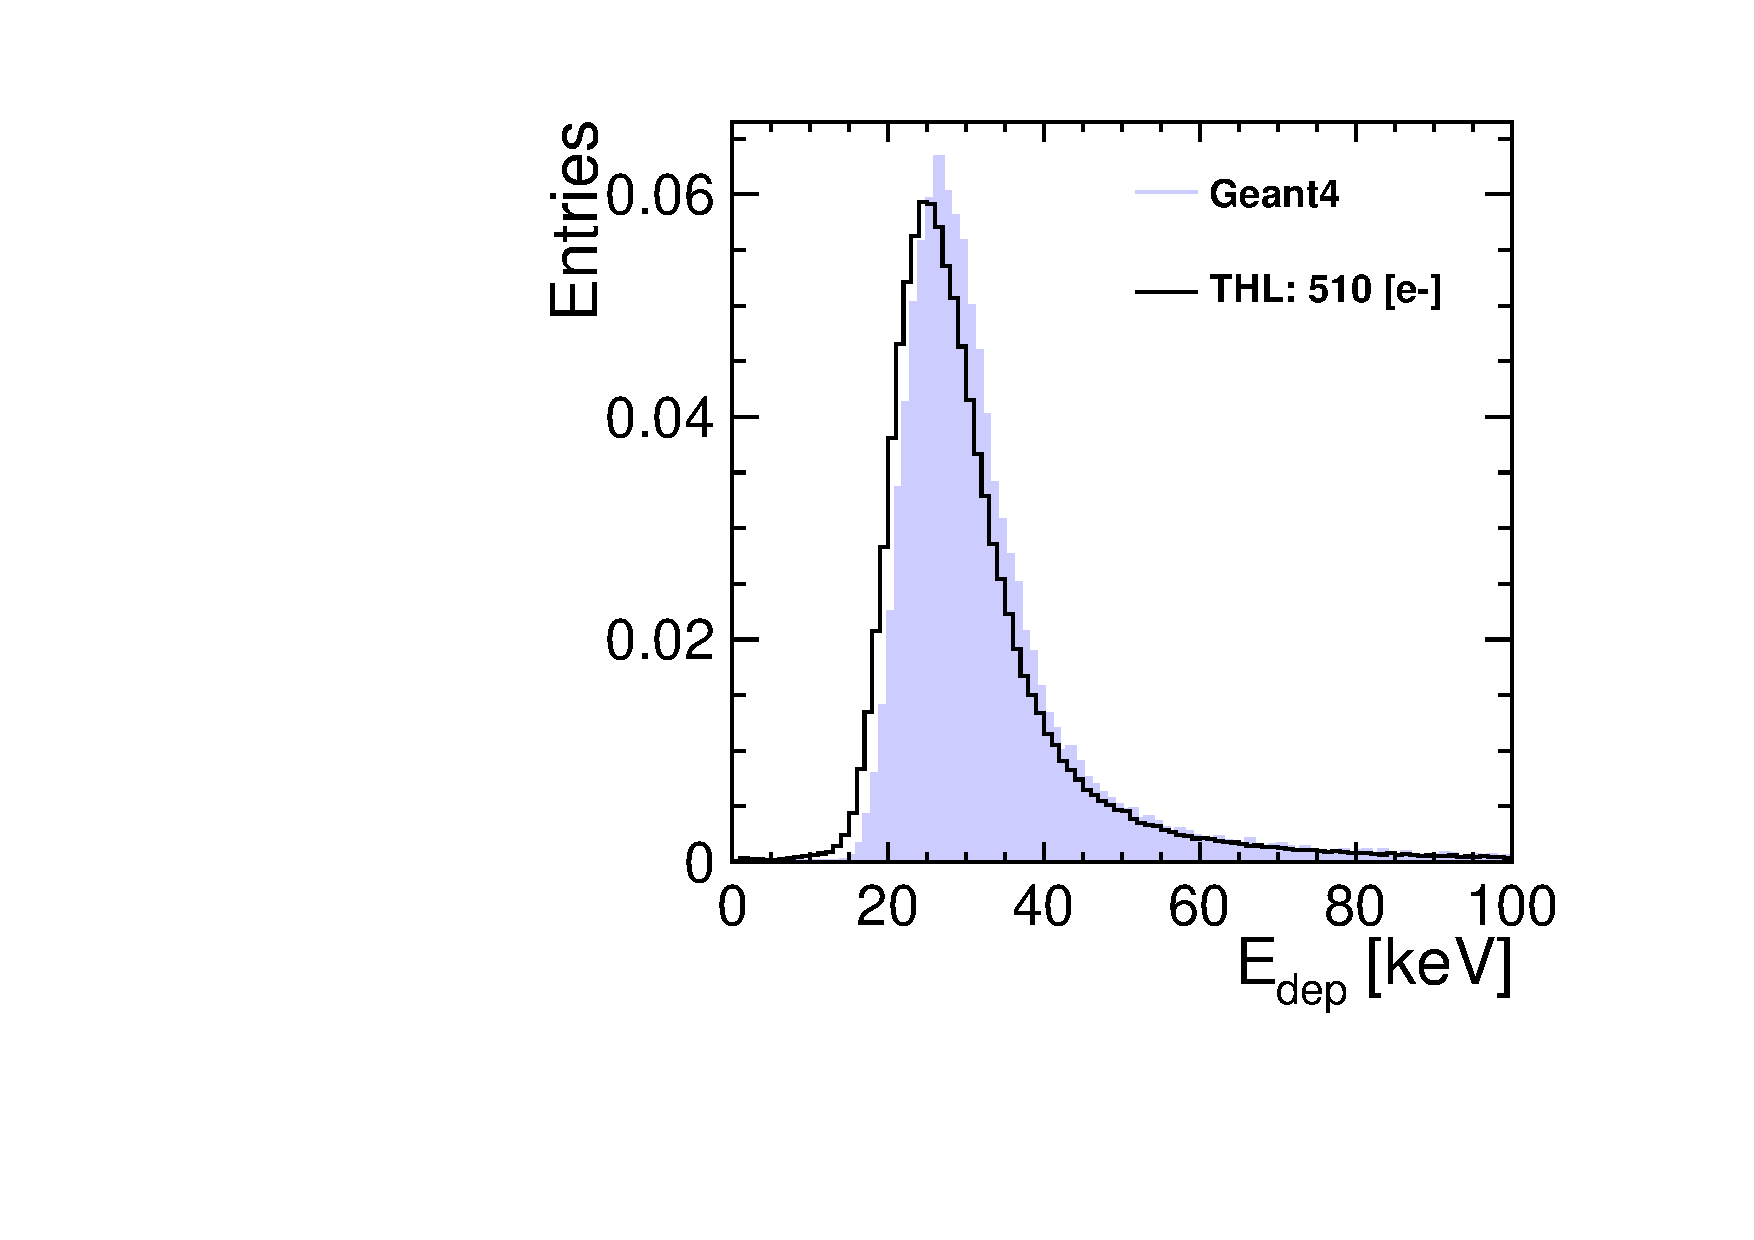
\includegraphics[width=\textwidth]{./figures/Calibration/Edep_G4_W0005_E02.pdf}
    \caption{}
  \end{subfigure}
  \caption{Energy deposition and comparison to
    \textsc{Geant4}. W0005\_E02, Run 661, THL=1160.}
  \label{fig:EdepW19L8}
\end{figure}

\begin{figure}[htbp] \centering
  \begin{subfigure}[b]{0.45\textwidth}
    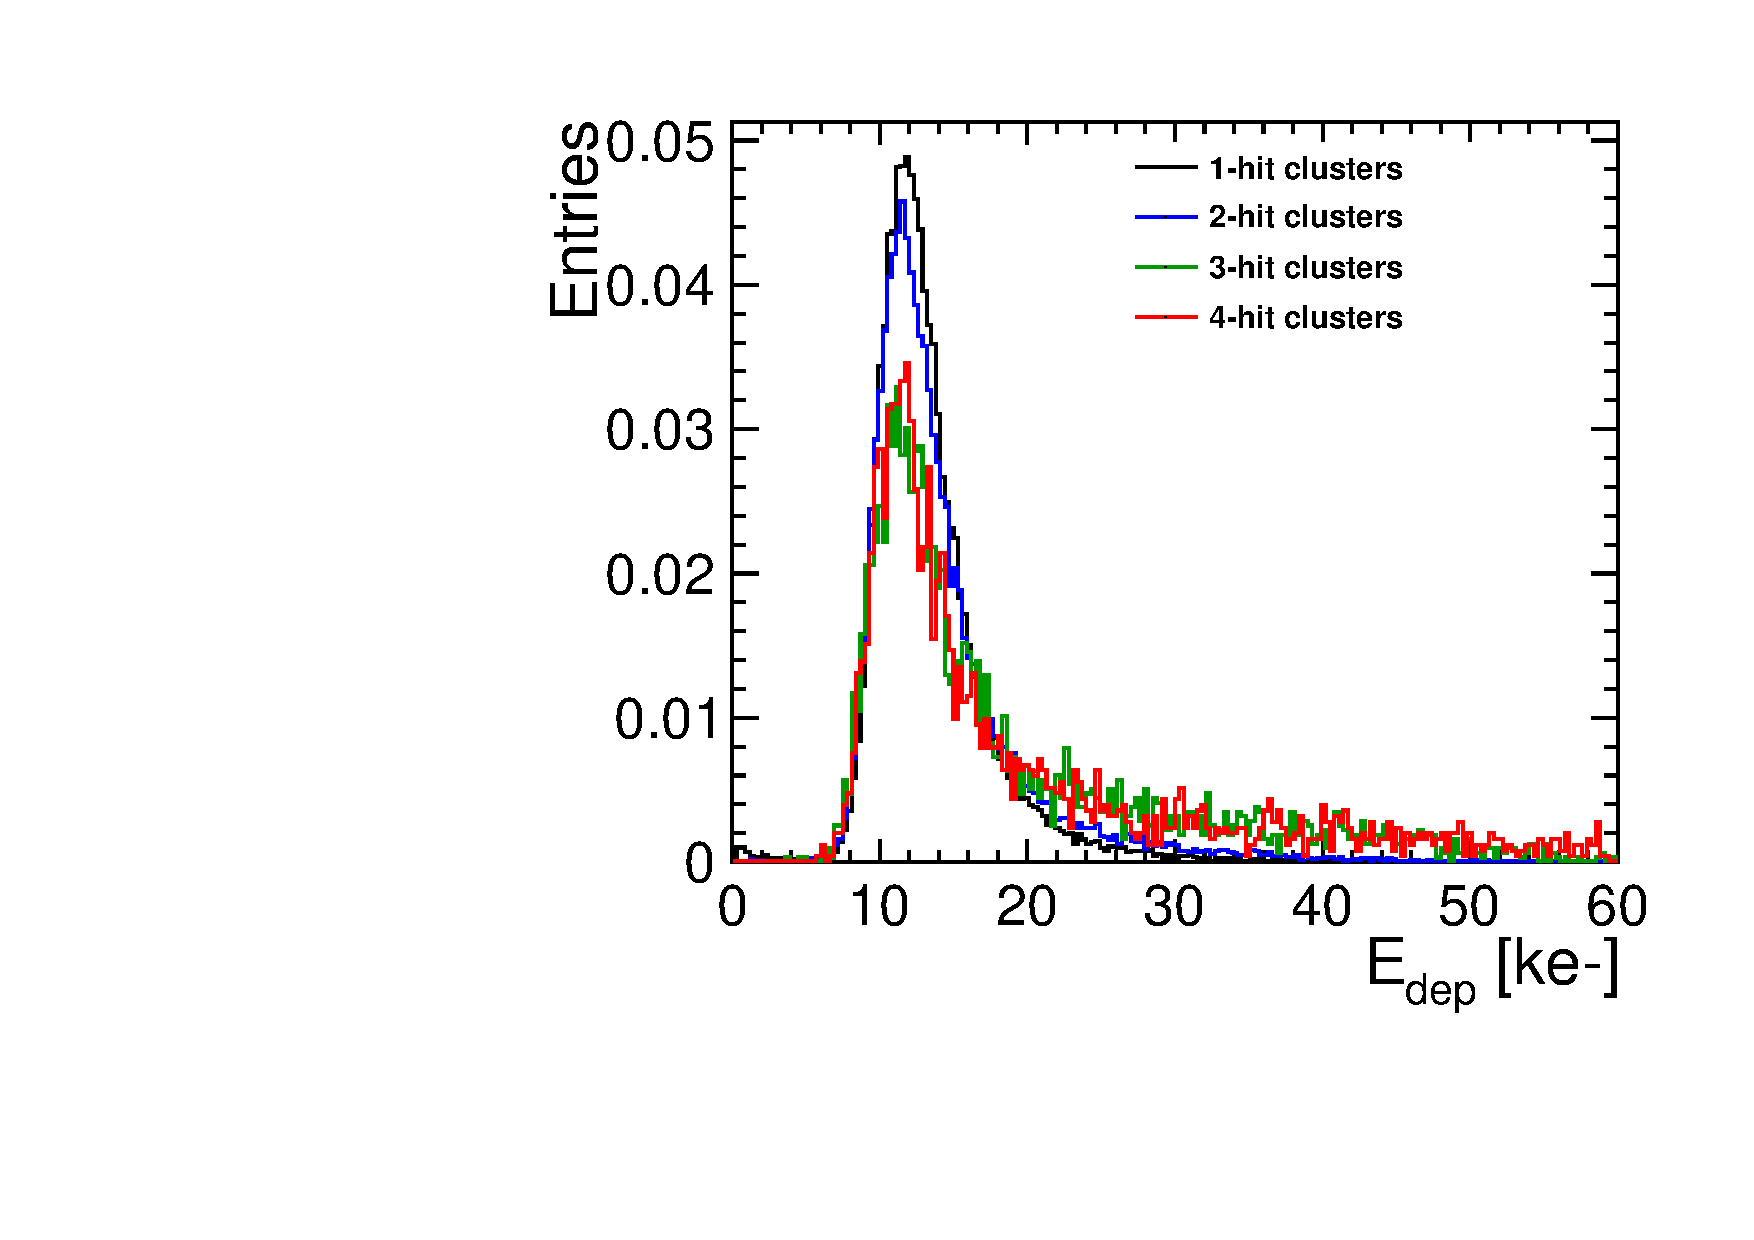
\includegraphics[width=\textwidth]{./figures/Calibration/Edep_Clusters_W0005_F01.pdf}
    \caption{}
  \end{subfigure}\hfill
  \begin{subfigure}[b]{0.45\textwidth}
    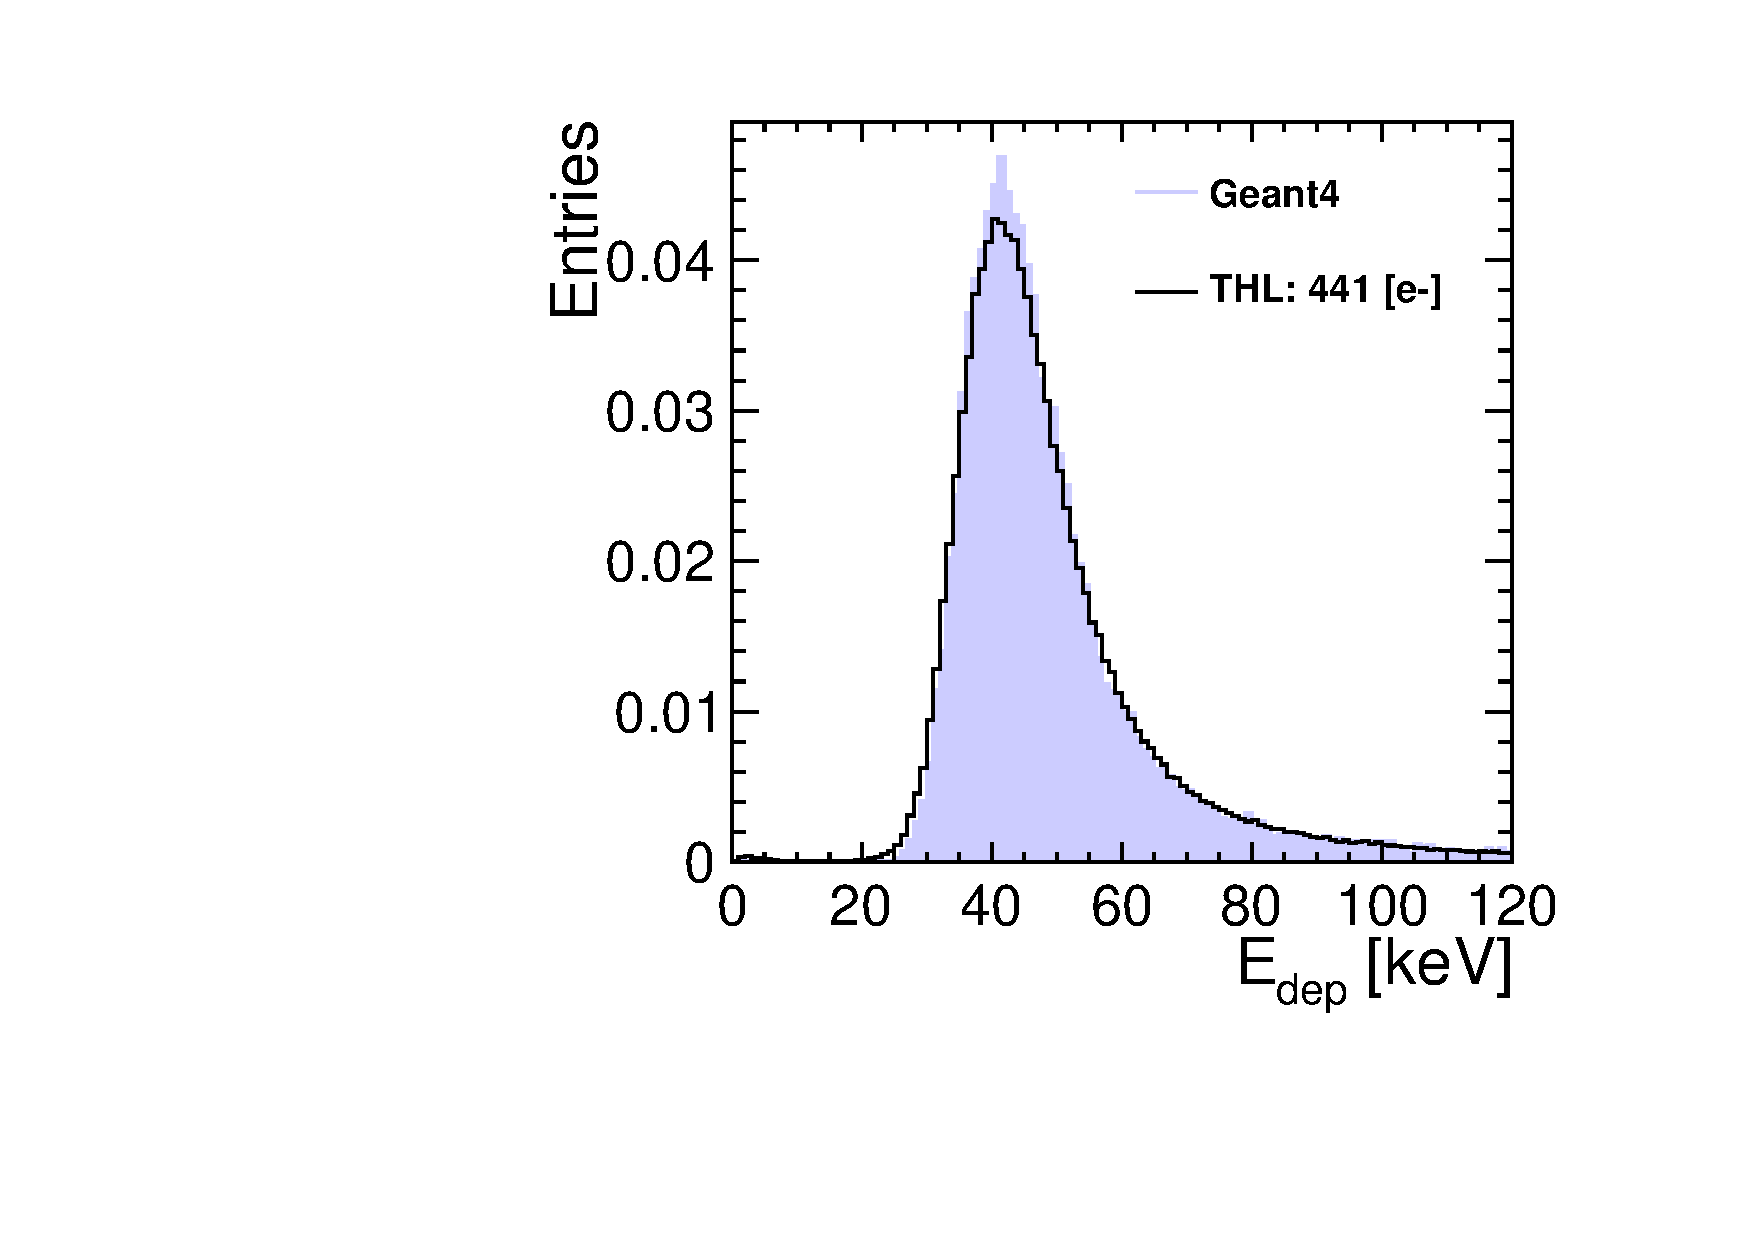
\includegraphics[width=\textwidth]{./figures/Calibration/Edep_G4_W0005_F01.pdf}
    \caption{}
  \end{subfigure}
  \caption{Energy deposition and comparison to
    \textsc{Geant4}. W0005\_F01, Run 761, THL=1153.}
  \label{fig:EdepW19L8}
\end{figure}

\subsection{Threshold calibration} \label{sec:threshold}


The operating threshold DAC (Digital-to-Analog Converter) set in each
Timepix/Timepix3 readout chip can be translated into an effective
energy and used as a data point for the surrogate fit at the
crossing-point on the $x$-axis. The counting (Medipix) mode was used
for this measurement. The assembly was exposed to photons of a
characteristic energy and the threshold DAC was scanned from a level
of no counts (threshold above the signal) to a level where all the
pixels count (threshold close to the noise level) resulting in an
S-shaped curve as shown in \cref{fig:scurve_example}. At the
maximum gradient of the S-curve, the threshold DAC corresponds to the
photon energy. The derivative of the S-curve is a Gaussian as shown in
\cref{fig:deriv_example} with a mean at the maximum gradient of
the S-curve. The derivative at each point of the S-curve corresponds
to the slope of the line connecting it to its neighbour.

\begin{figure}[htbp] \centering
  \begin{subfigure}[b]{0.45\textwidth}
    \begin{tikzpicture} \node[anchor=south west,inner sep=0] (image)
      at
      (0,0){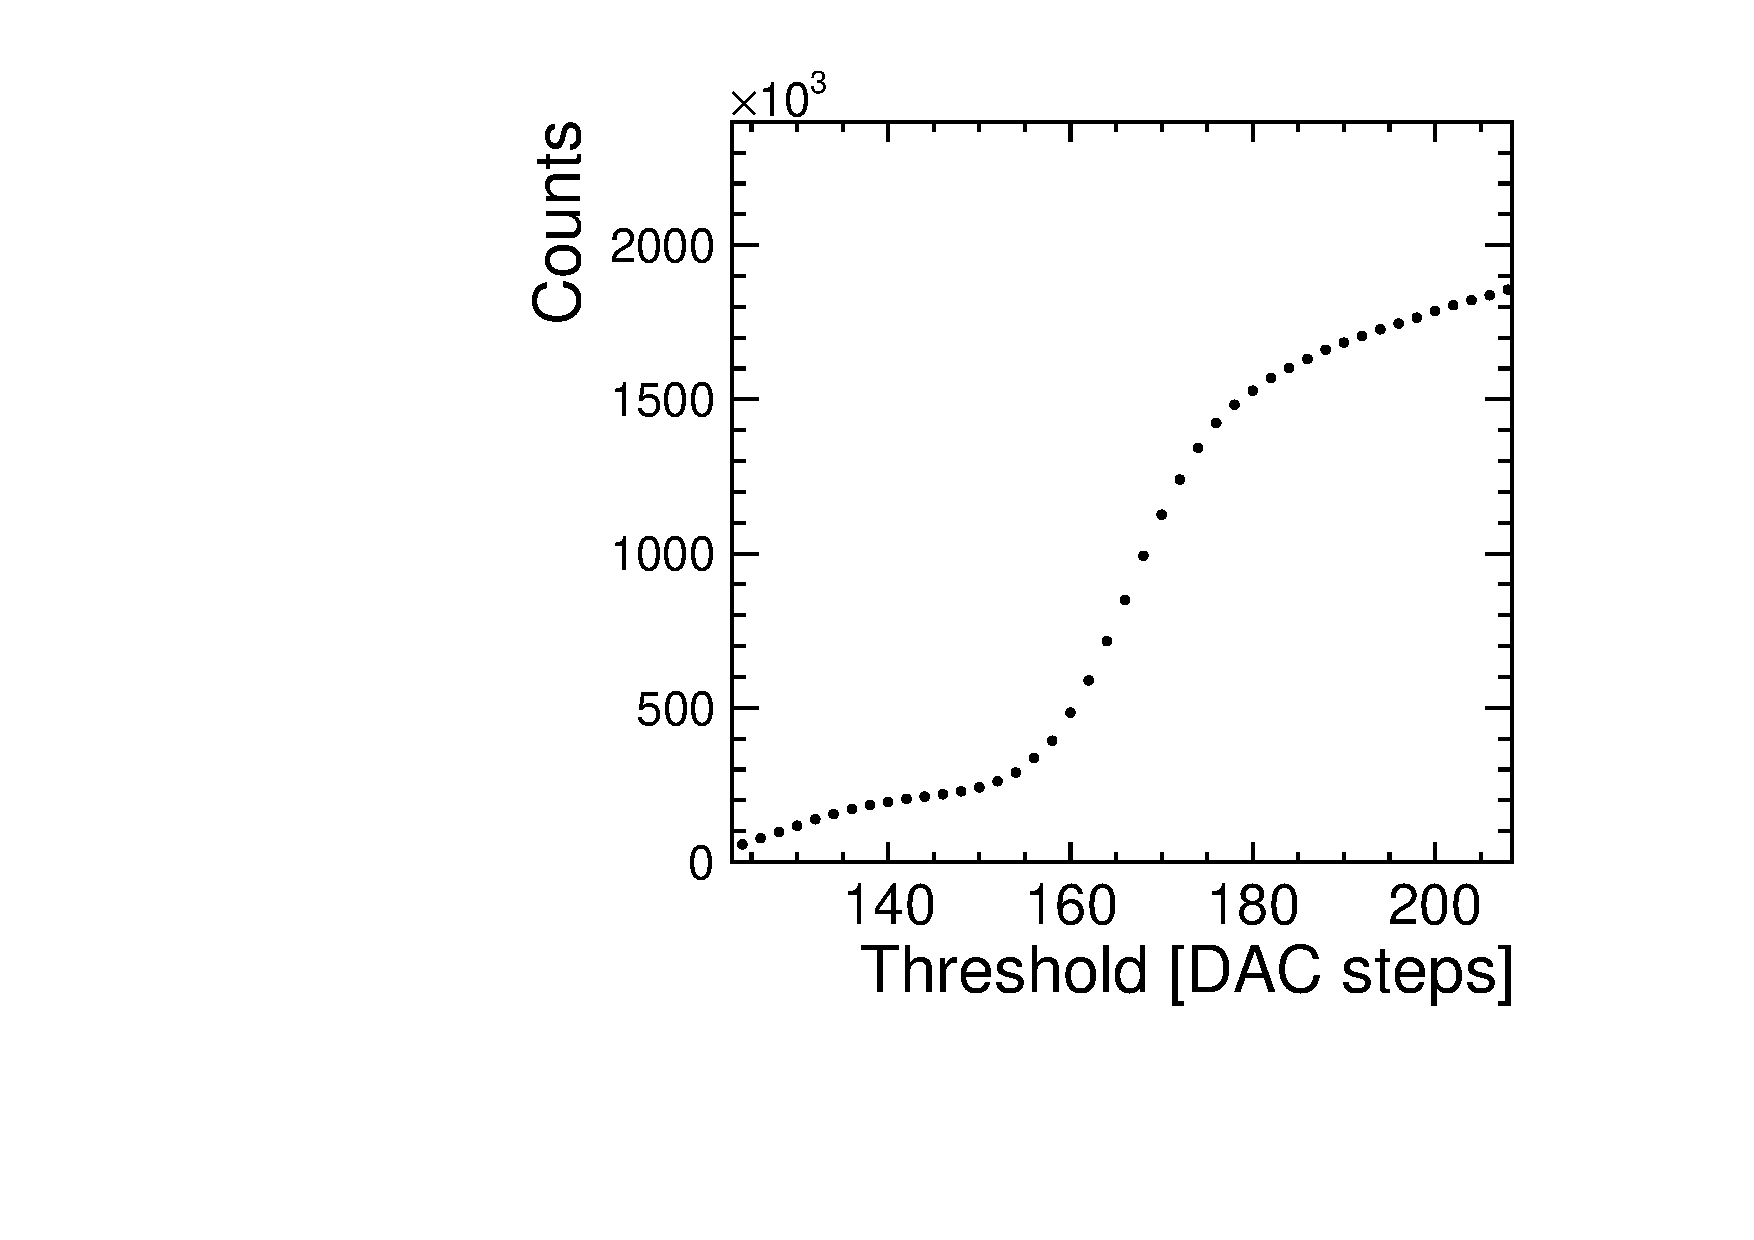
\includegraphics[width=\textwidth]{./figures/Calibration/L04-W0125_scurve_In.pdf}};
      % \draw[->,line width=.4pt, color=black](1.8, 1.4) -- (2.4, 1.4);
      \node[left, color=black] at (1.9, 1.6) {$K_{\beta}$}; %\draw[->,line
      width=.4pt, color=black](3, 2.7) -- (3.7, 2.7); \node[left,
      color=black] at (3.5, 2.7) {$K_{\alpha}$};
    \end{tikzpicture}
    \caption{Measured S-curve}
    \label{fig:scurve_example}
  \end{subfigure} \hfill
  \begin{subfigure}[b]{0.45\textwidth}
    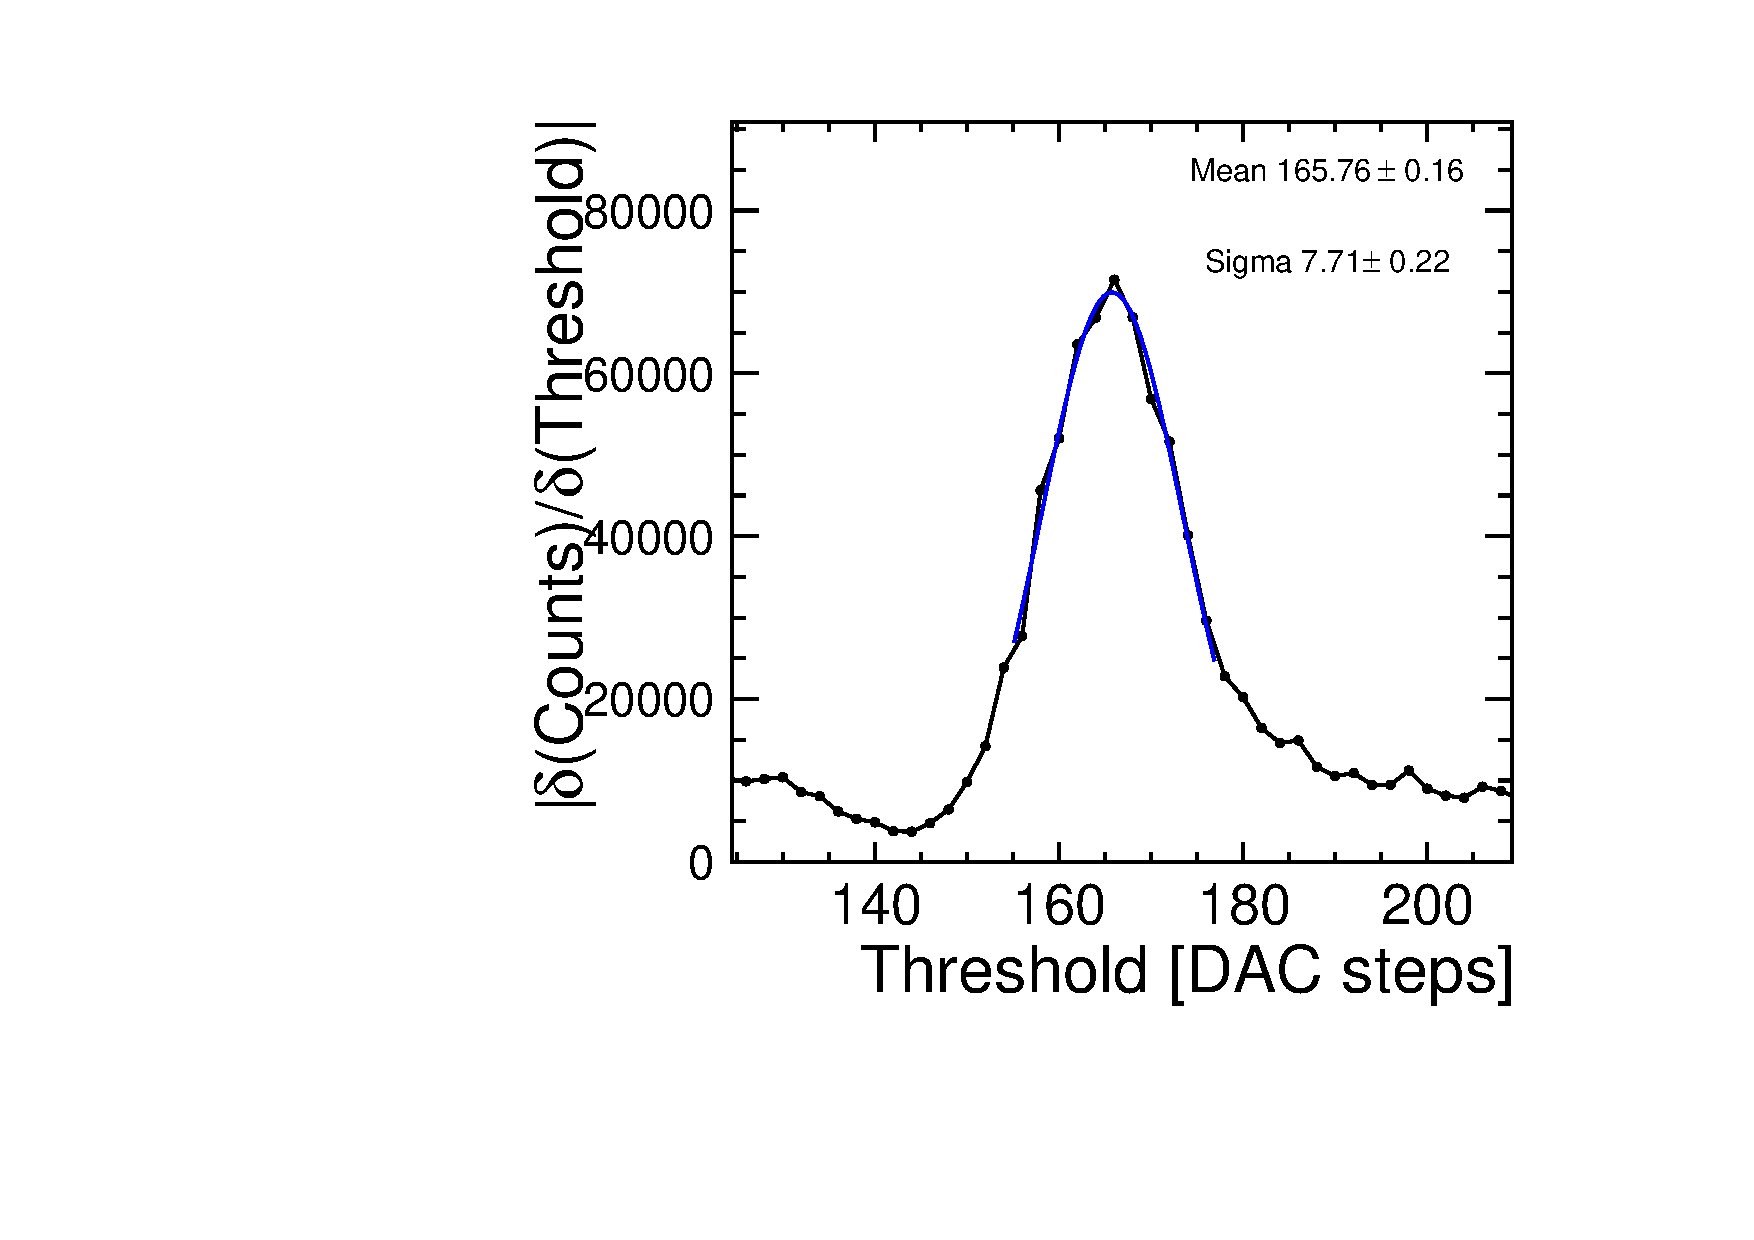
\includegraphics[width=\textwidth]{./figures/Calibration/L04-W0125_scurveDeriv_In.pdf}
    \caption{Derivative of the S-curve}
    \label{fig:deriv_example}
  \end{subfigure}
  \caption{An example of a measured S-curve (a) and its derivative
    fitted with a Gaussian function (b) for L04-W0125 (Timepix readout
    ASIC) using the Indium target. $K_{\alpha}$ corresponds to the
    strongest X-ray spectral line for the bombarded target. The smaller
    peak for $K_{\beta}$ is ignored. For Timepix assemblies. The Pixelman
    software~\cite{1748-0221-6-01-C01046} provides the \emph{DACs Scan}
    plug-in which was used to scan the threshold DAC value and save the
    hit maps in a text file. The threshold calibration was done at CERN
    using the XRF targets. This measurement was performed globally for
    each assembly. The threshold DAC is scanned with a step size of 2.}
  \label{fig:scurve_deriv_example}
\end{figure}

A linear fit was used to parametrise the relationship between the
photon energy and the threshold DAC given by the mean of the
derivative of the S-curves:
\begin{equation}
  THL_{DAC}=p \; THL_{\kev} + q \; ,
  \label{eq:THLDAC}
\end{equation}
where $THL_{DAC}$ is the threshold DAC and $THL_{\kev}$ its conversion
into an energy. \cref{fig:THLcalib_A06} shows an example of the
threshold calibration obtained for A06-W0110. Each point used for the
fit corresponds to the mean of the Gaussian fitted to the derivative
of the S-curve for each target. The error on each point corresponds to
the error on the mean of the fitted Gaussian.

\begin{figure}[htbp]
  \centering
  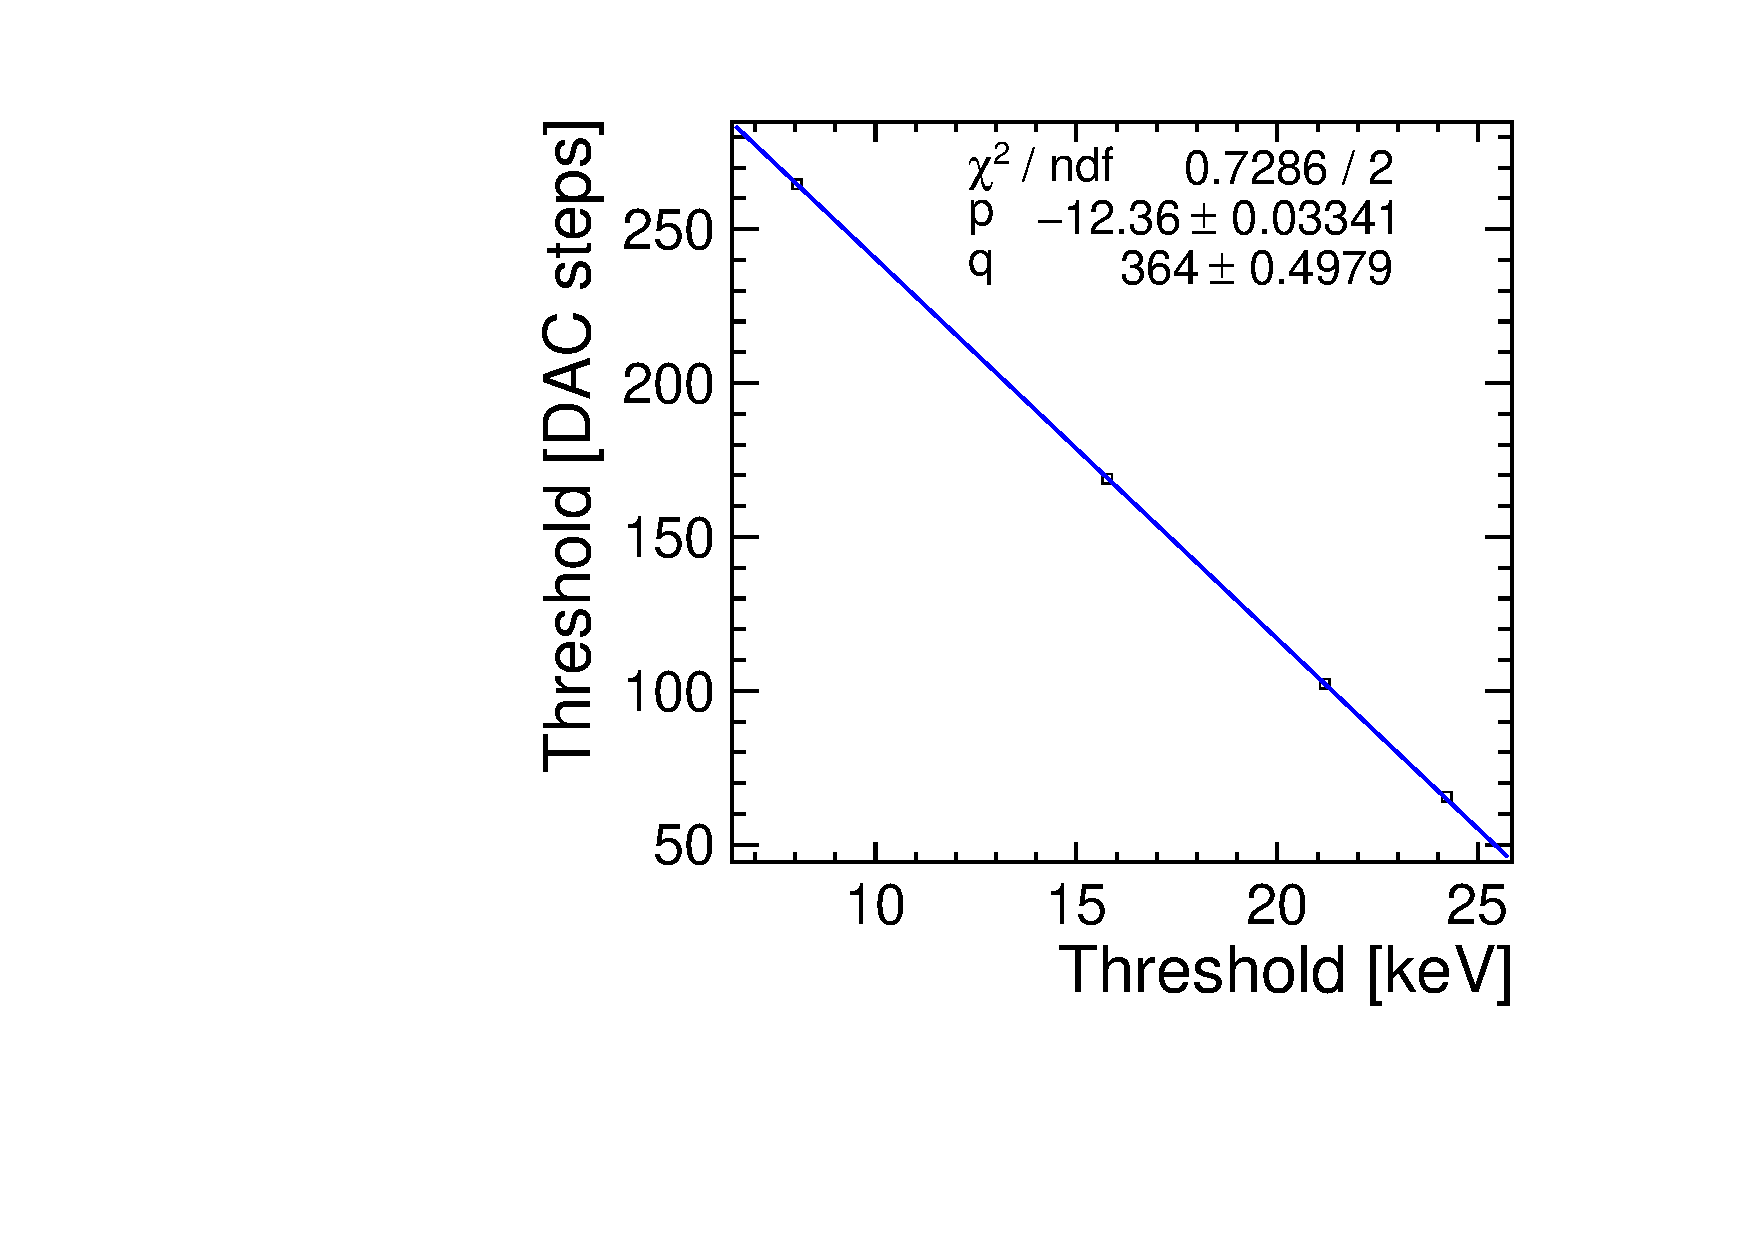
\includegraphics[width=0.5\textwidth]{./figures/Calibration/A06-W0110_THLcalibration.pdf}
  \caption{Threshold calibration for A06-W0110. Each point corresponds
    to the maximum gradient of the S-curve for each target (Cu, Zr, Pd
    and In). A linear function as described in \cref{eq:THLDAC} was
    used to fit the data points and obtain the parameters $p$ and
    $q$.}
  \label{fig:THLcalib_A06}
\end{figure}

The operating threshold DAC for each assembly was converted to an
energy by solving \cref{eq:THLDAC} for $THL_{\kev}$ with
$THL_{DAC}=THL_{DAC}^{op}$. Results are shown in \cref{tab:evalTHL}. The error on the evaluated threshold in energy
($THL_{\kev}^{op}$) is obtained by the propagation of errors for the
inverse of \ref{eq:THLDAC}:
\begin{equation}
  \sigma_{THL_{\kev}}^2(THL_{DAC})={{{(THL_{DAC}-q)^2} \over {p^4}} \sigma_{p}^2} +
        {\frac{1}{p^2} \sigma_{q}^2}+
        {2 {{THL_{DAC}-q} \over p^3} \sigma_{pq}^2} \; ,
        \label{eq:THLerror}
\end{equation}
where $p$, $q$ are given by the linear fit using \cref{eq:THLDAC} with
standard deviations $\sigma_{p}$, $\sigma_{q}$ and covariance
$\sigma_{pq}$.

\begin{table}[htbp]
  \caption{Threshold fit parameters $p$ and $q$, the operating
    threshold DAC and its conversion into energy.}
  \label{tab:evalTHL} 
  \centering
  \begin{tabular}{ c c c c c }
    \toprule
    Assembly & $p$ [DAC steps/\kev] & $q$ [DAC steps] & $THL_{DAC}^{op}$ [DAC steps] & $THL_{\kev}^{op}$ [\kev] \\
    \midrule
    A06-W0110 & $-12.36\pm0.03$ & $364.0\pm0.50$ & 326 & $3.077\pm0.033$ \\
    C04-W0110 & $-11.8\pm0.02$ & $441.6\pm0.42$ & 405 & $3.102\pm0.030$ \\
    L04-W0125 & $-11.68\pm0.02$ & $448.6\pm0.31$ & 410 & $3.303\pm0.023$ \\
    B06-W0125 & $11.58\pm0.037$ & $390.6\pm0.80$ & 435 & $3.836\pm0.057$ \\
    \bottomrule
  \end{tabular}
\end{table}

For further verification of these results, the DAC step gain for each
assembly was calculated to be around
24~$\pm$e\textsuperscript{-}/step, in agreement
with~\cite{art:tmpx}. The width of the derivative of the S-curves
shows the error at the front-end of the assembly. For all assemblies
it varies between 7 to 11 DAC values which corresponds to 170 to 270
electrons, again in agreement with~\cite{art:tmpx} (the error is
obtained by error propagation of \cref{eq:THLDAC}).


\subsection{Threshold calibration with test pulses}

The Timepix readout chips provide an internal test pulse generator
which can be used for calibration as well as equalisation of the
readout chip. In each pixel, a capacitor allows for injecting a charge
by switching a voltage over it. The charge injected is given by
\cref{eq:testpulseCharge}:

\begin{equation}
  Q = C \cdot \Delta V
  \label{eq:testpulseCharge}
\end{equation}

where Q is the injected charge, C the injection capacitance and
$\Delta V$ the voltage applied. A priori, the injection capacitance is
unknown and its value varies a lot from pixel to pixel but its value
can be measured (HOW?). 
For the Timepix3 readout chip, the test pulse calibration gives very
good results and is used to calibrate the threshold as well as the TOT
and the TOA. 

For the calibration of the threshold, pulses at four different heights
are injected (at 0, 1000, 3000 and 6000
electrons). \cref{fig:Timepix3_THL_Calibration} shows the threshold
calibration for different assemblies. 



\begin{table}[htbp]
  \centering
  \caption{Advacam active-edge n-in-p planar pixel sensor assemblies. The edge distance is defined by the distance between the last pixel implant and the physical sensor edge.}
  \label{tab:NominalThreshold}
  \begin{tabular}{lccc}
    \toprule
    Assembly & Nominal THL\textsubscript{DAC}\textsuperscript{op} [DAC steps] & Nominal THL\textsubscript{e-}\textsuperscript{op} [electrons]\\
    \midrule
    W19\_G7 & 1190 & 466.5\\
    W19\_F7 & 1187 & 532.4\\ \hline
    W19\_L8 & 1133 & 517.8\\
    W19\_C7 & 1148 & 553.7\\
    W5\_E2 & 1160 & 537.9\\ \hline
    W5\_F1 & 1153 & 441.2\\
    \bottomrule
  \end{tabular}
\end{table}


TODO:\\ 
- Explain method\\
- make a table with nominal operating threshold\\
- Calculate errors with the error propagation\\


\begin{figure}[htbp] \centering
  \begin{subfigure}[b]{0.45\textwidth}
    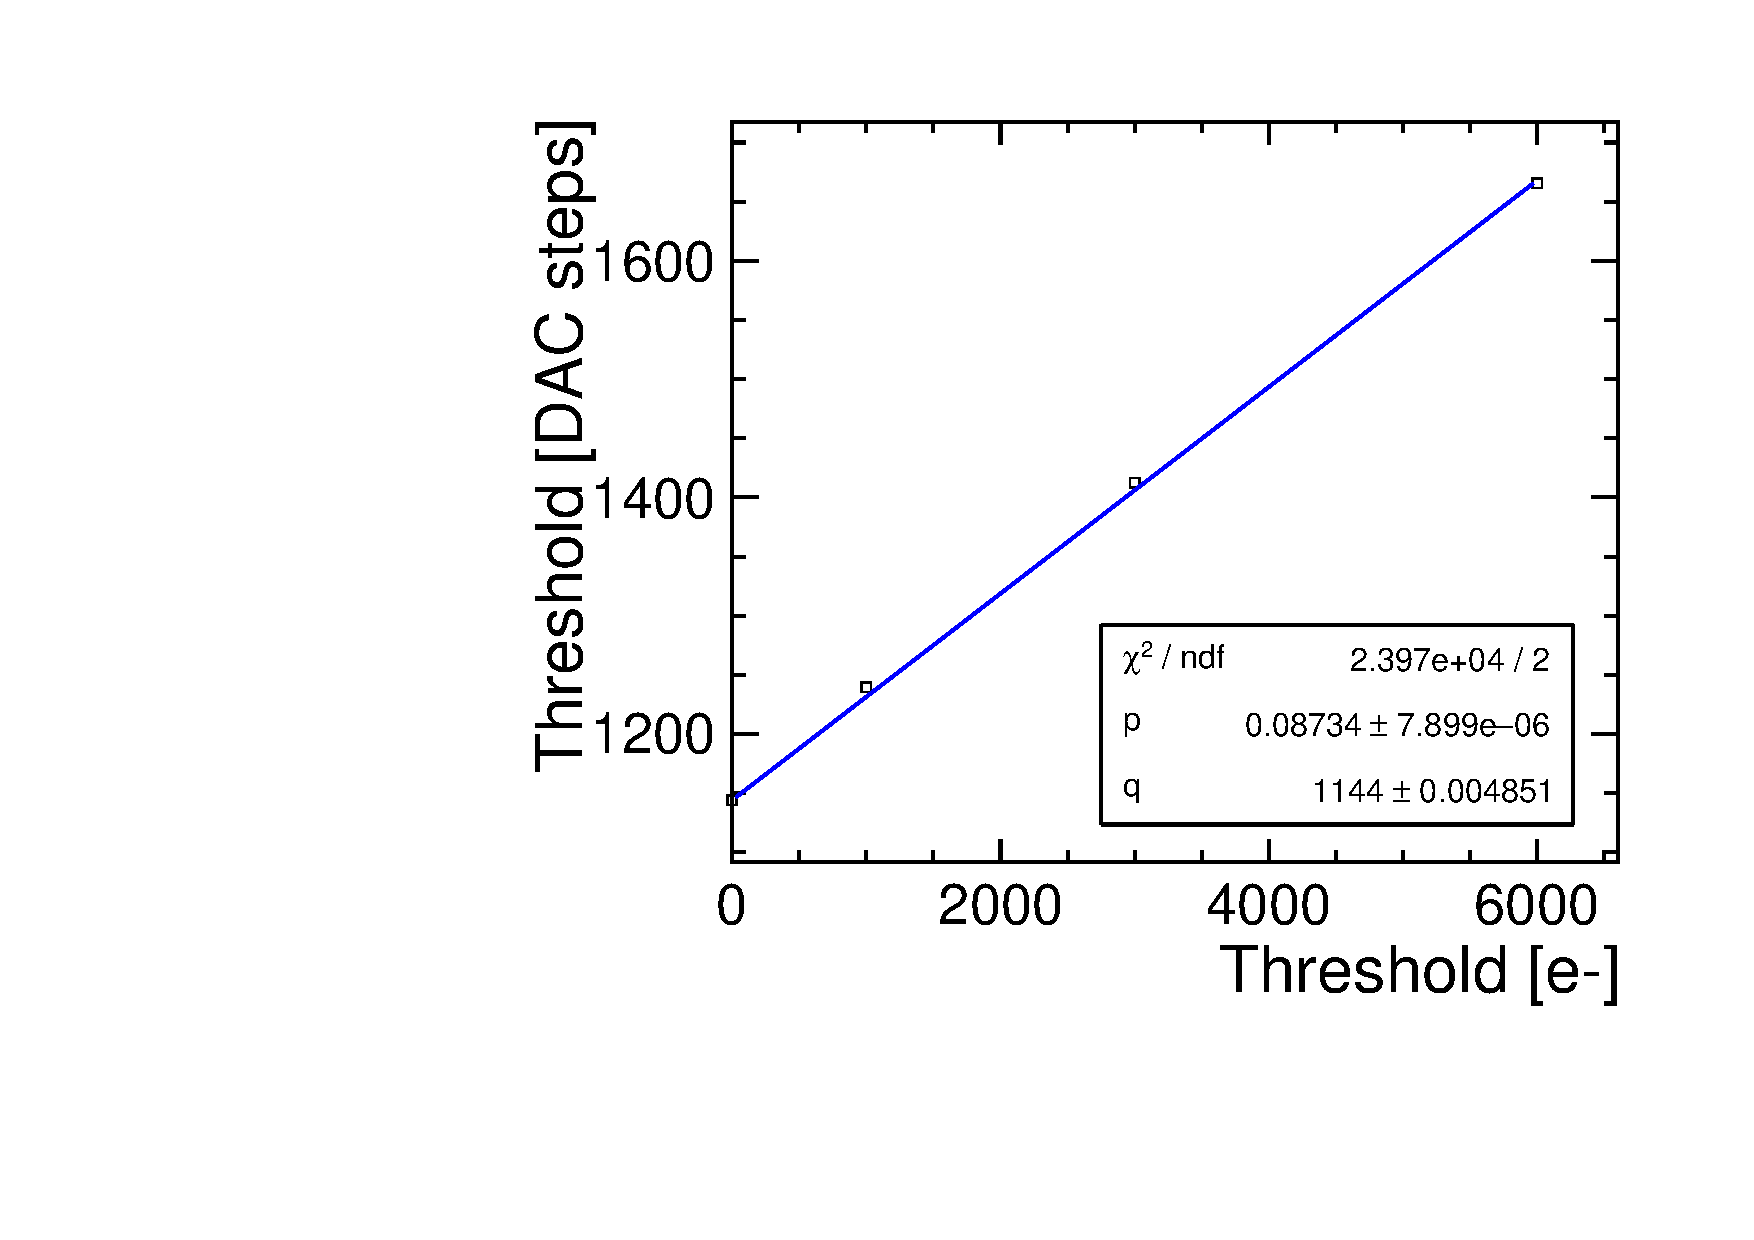
\includegraphics[width=\textwidth]{./figures/Calibration/THLcalibration_W0019_G07.pdf}
    \caption{20-NGR}
  \end{subfigure} \hfill
  \begin{subfigure}[b]{0.45\textwidth}
    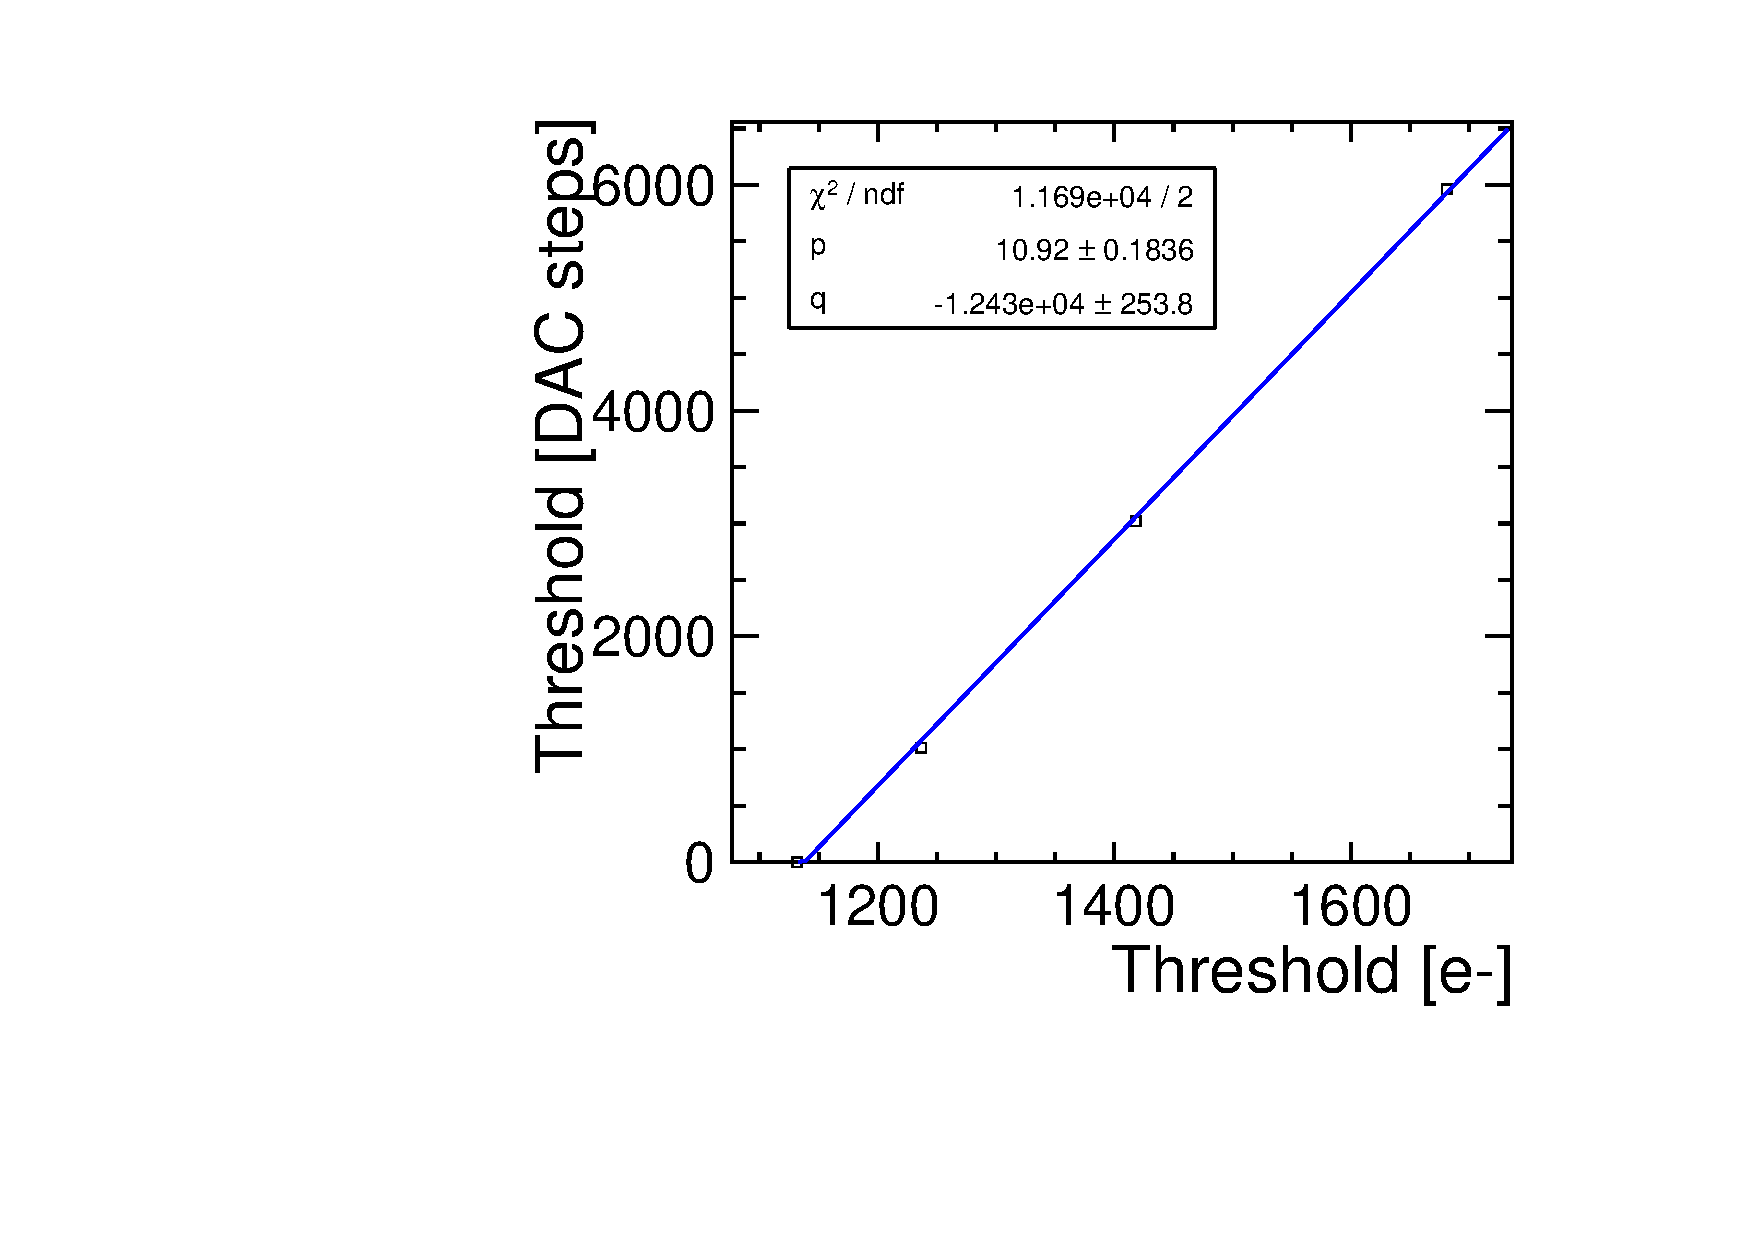
\includegraphics[width=\textwidth]{./figures/Calibration/THLcalibration_W0019_F07.pdf}
    \caption{23-FGR}
  \end{subfigure}\\
  \begin{subfigure}[b]{0.45\textwidth}
    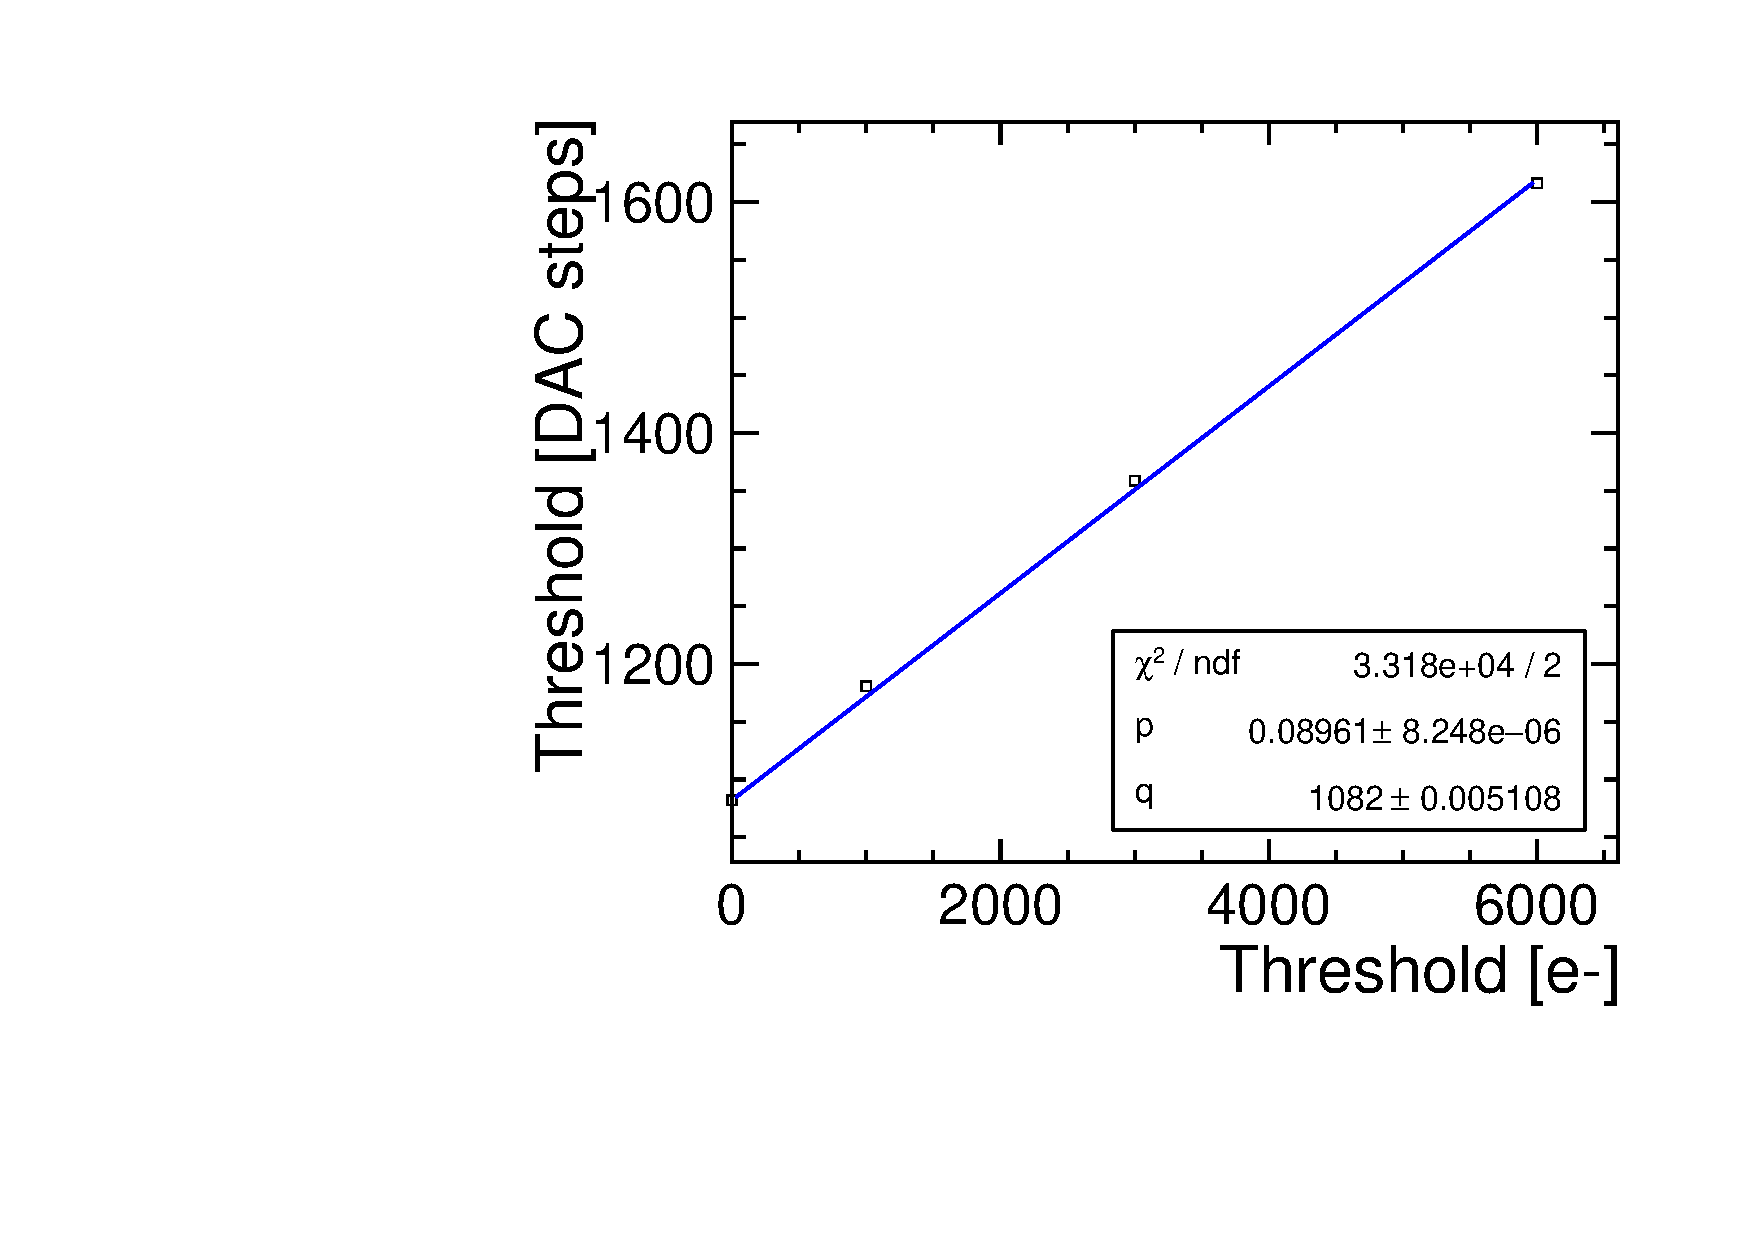
\includegraphics[width=\textwidth]{./figures/Calibration/THLcalibration_W0019_L08.pdf}
    \caption{28-GNDGR}
  \end{subfigure} \hfill
  \begin{subfigure}[b]{0.45\textwidth}
    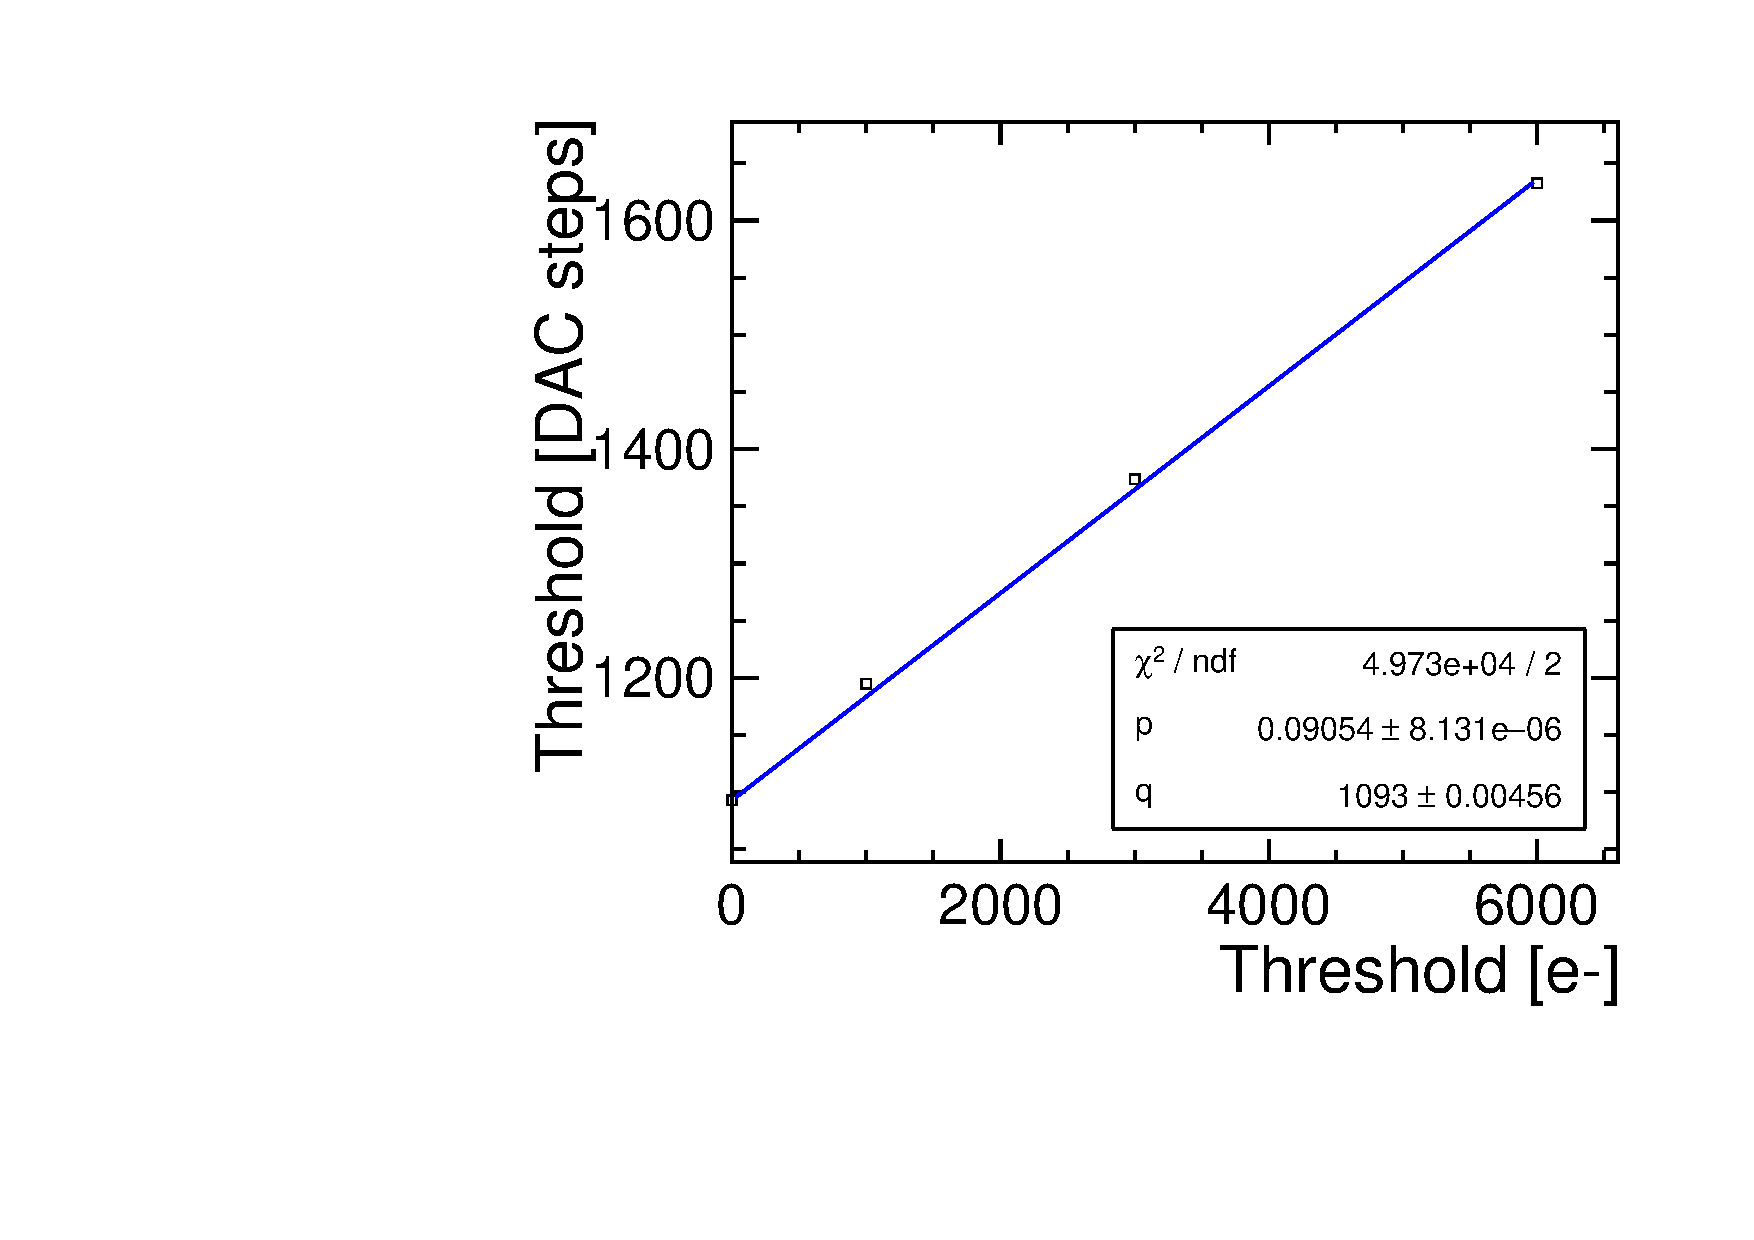
\includegraphics[width=\textwidth]{./figures/Calibration/THLcalibration_W0019_C07.pdf}
    \caption{55-GNDGR}
  \end{subfigure}\\
  \begin{subfigure}[b]{0.45\textwidth}
    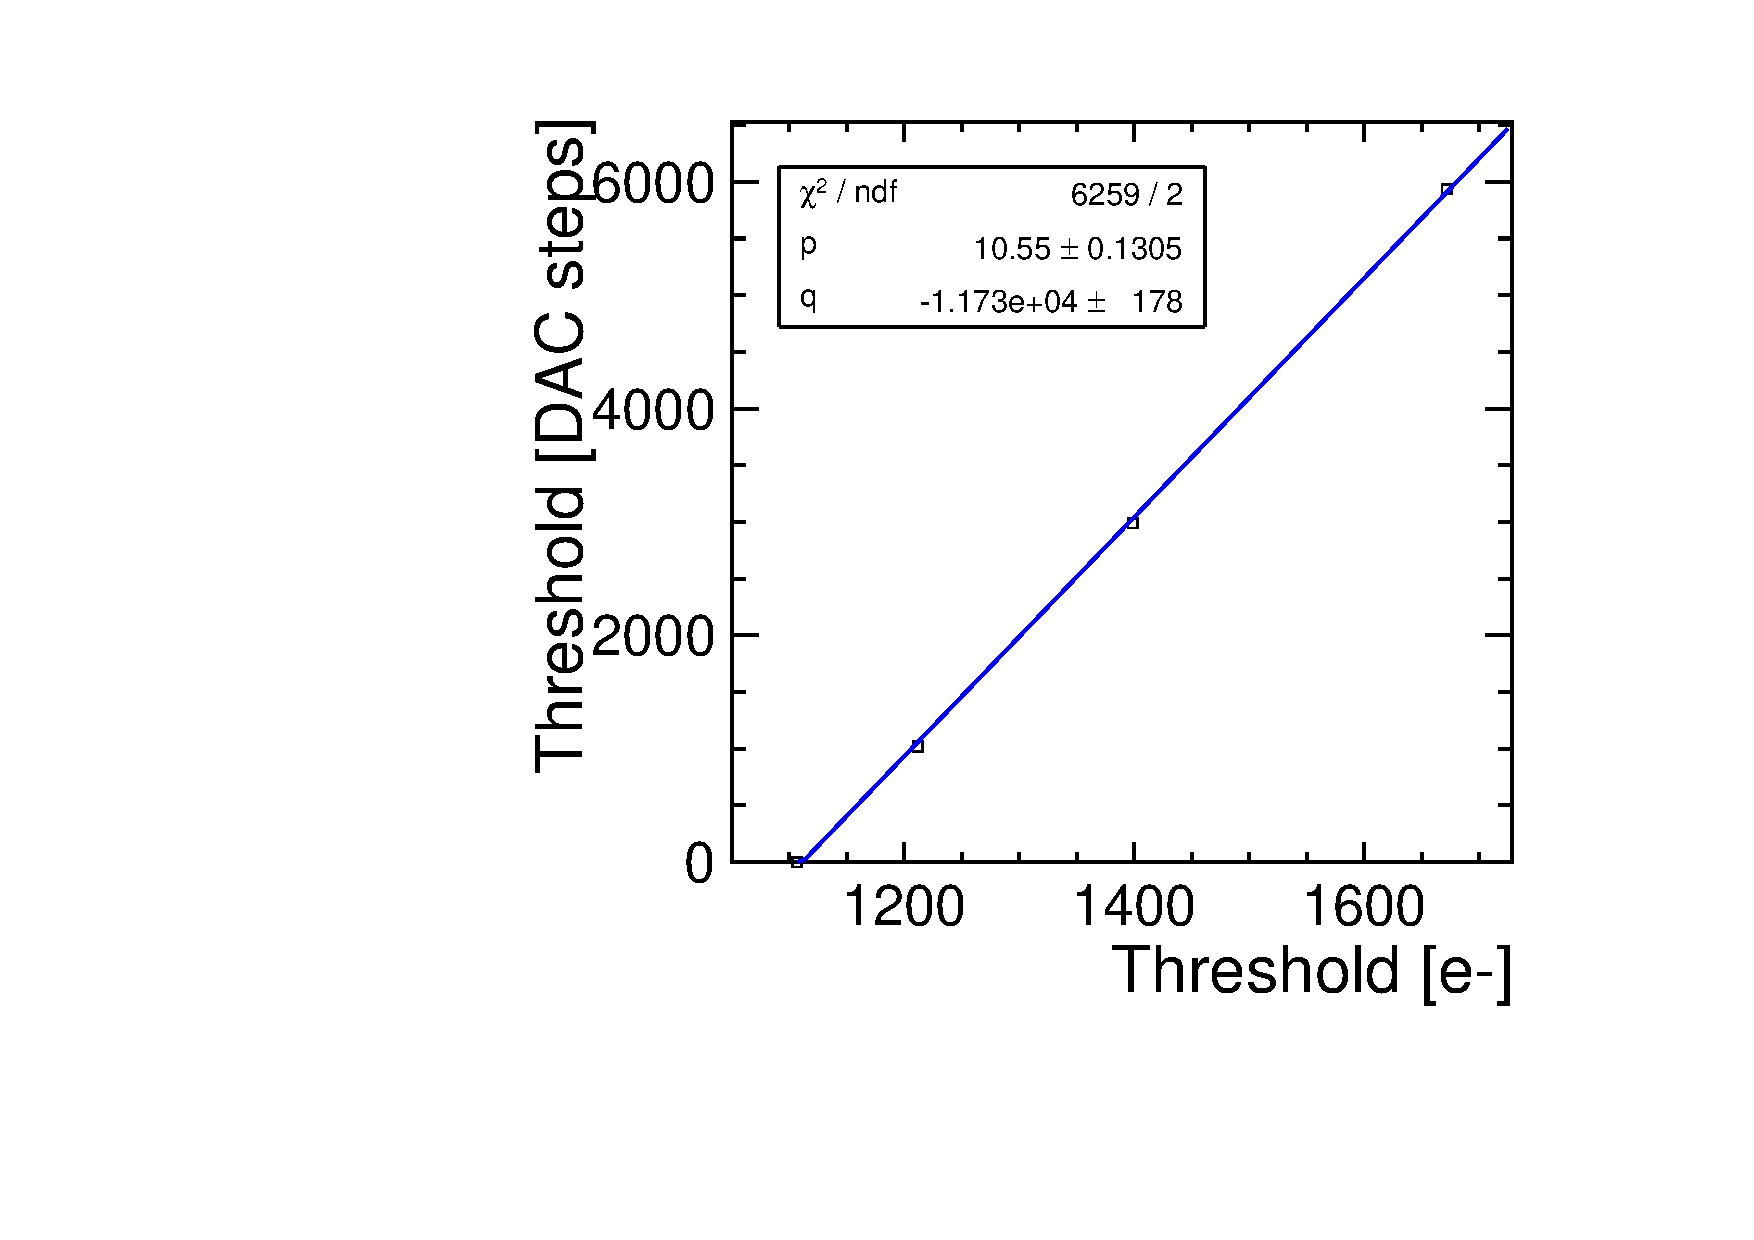
\includegraphics[width=\textwidth]{./figures/Calibration/THLcalibration_W0005_E02.pdf}
    \caption{55-GNDGR-100}
  \end{subfigure} \hfill
  \begin{subfigure}[b]{0.45\textwidth}
    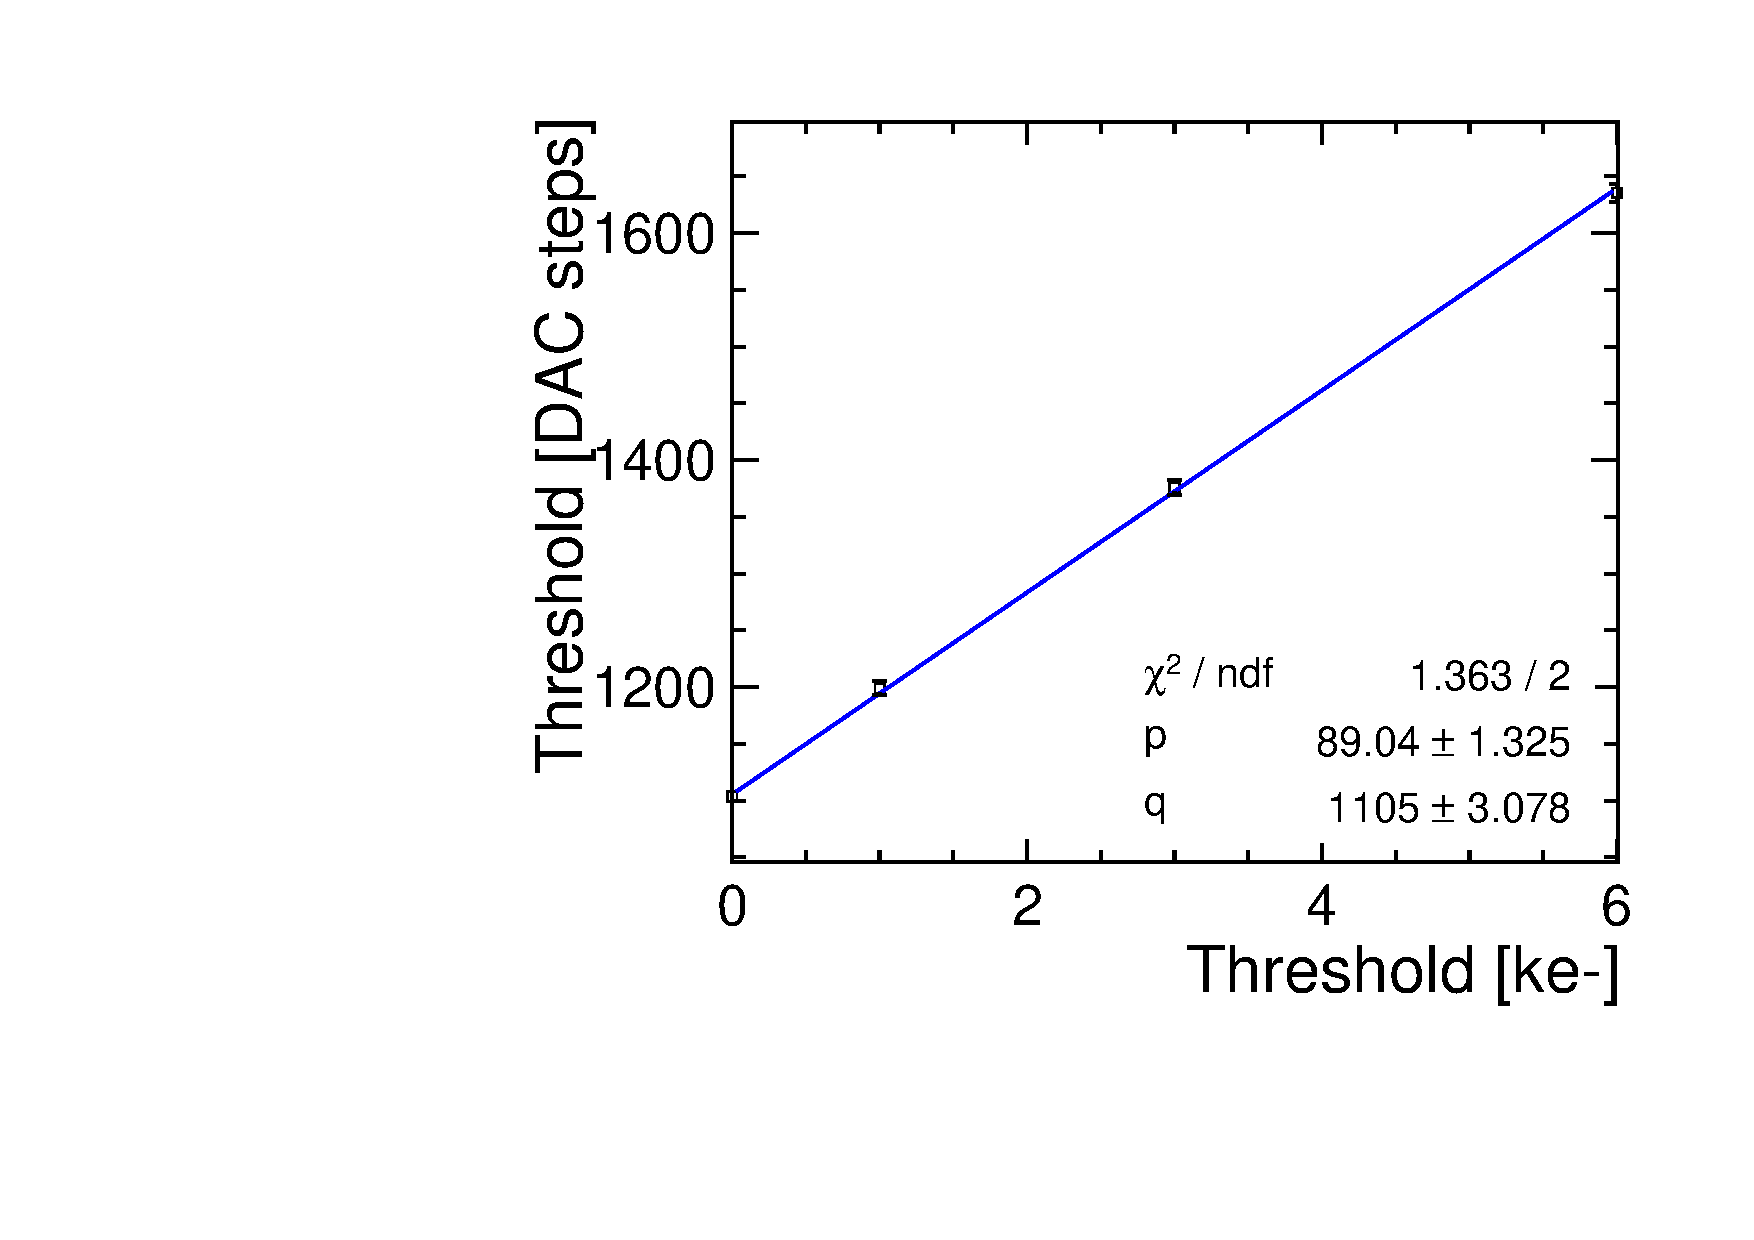
\includegraphics[width=\textwidth]{./figures/Calibration/THLcalibration_W0005_F01.pdf}
    \caption{55-GNDGR-150}
  \end{subfigure}
  \caption{Threshold calibration for Timepix3 assemblies using test pulses.}
  \label{fig:Timepix3_THL_Calibration}
\end{figure}

%%%%%%%%%%%%%%%%%%%%%%%%%%%%%%%%%%%%%%%%%%%%%%%%%%%%%%%%
%%%%%%%%%%%%%%%%%%%%%%%%%%%%%%%%%%%%%%%%%%%%%%%%%%%%%%%%
%%%%%%%%%%%%%%%%%%%%%%%%%%%%%%%%%%%%%%%%%%%%%%%%%%%%%%%%
% \begin{table}[htbp]
%   \caption{Measured DAC step gain.}
%   \label{tab:DACStep}
%   \centering
%   \begin{tabular}{ c c c }
%     \toprule
%     Assembly & Threshold DAC step [\ev] & Threshold DAC step [\Pem] \\
%     \midrule
%     A06-W0110  & $81\pm0.009$ & $22.475\pm0.025$  \\
%     C04-W0110  & $85\pm0.039$ & $23.544\pm0.011$ \\
%     L04-W0125 &  $86\pm0.022$ & $23.775\pm0.006$ \\
%     B06-W0125  & $86\pm0.120$ & $23.978\pm0.033$ \\
%     \bottomrule
%   \end{tabular}
% \end{table}

% Threshold measurements were not completed for assemblies B07-W0125 and
% D09-W0126. Assembly B07-W0125 did not fully deplete due to a broken
% corner of the sensor. The derivative of the CuXRF S-curve did not form
% a peak as the photon energy was close to the noise level. Assembly
% D09-W0126 was not operating as expected for a $100\,\micron$
% sensor. Therefore the calibration of these assemblies was done without
% threshold measurements.